% Options for packages loaded elsewhere
\PassOptionsToPackage{unicode}{hyperref}
\PassOptionsToPackage{hyphens}{url}
%
\documentclass[
]{book}
\usepackage{amsmath,amssymb}
\usepackage{lmodern}
\usepackage{iftex}
\ifPDFTeX
  \usepackage[T1]{fontenc}
  \usepackage[utf8]{inputenc}
  \usepackage{textcomp} % provide euro and other symbols
\else % if luatex or xetex
  \usepackage{unicode-math}
  \defaultfontfeatures{Scale=MatchLowercase}
  \defaultfontfeatures[\rmfamily]{Ligatures=TeX,Scale=1}
\fi
% Use upquote if available, for straight quotes in verbatim environments
\IfFileExists{upquote.sty}{\usepackage{upquote}}{}
\IfFileExists{microtype.sty}{% use microtype if available
  \usepackage[]{microtype}
  \UseMicrotypeSet[protrusion]{basicmath} % disable protrusion for tt fonts
}{}
\makeatletter
\@ifundefined{KOMAClassName}{% if non-KOMA class
  \IfFileExists{parskip.sty}{%
    \usepackage{parskip}
  }{% else
    \setlength{\parindent}{0pt}
    \setlength{\parskip}{6pt plus 2pt minus 1pt}}
}{% if KOMA class
  \KOMAoptions{parskip=half}}
\makeatother
\usepackage{xcolor}
\usepackage{color}
\usepackage{fancyvrb}
\newcommand{\VerbBar}{|}
\newcommand{\VERB}{\Verb[commandchars=\\\{\}]}
\DefineVerbatimEnvironment{Highlighting}{Verbatim}{commandchars=\\\{\}}
% Add ',fontsize=\small' for more characters per line
\usepackage{framed}
\definecolor{shadecolor}{RGB}{248,248,248}
\newenvironment{Shaded}{\begin{snugshade}}{\end{snugshade}}
\newcommand{\AlertTok}[1]{\textcolor[rgb]{0.94,0.16,0.16}{#1}}
\newcommand{\AnnotationTok}[1]{\textcolor[rgb]{0.56,0.35,0.01}{\textbf{\textit{#1}}}}
\newcommand{\AttributeTok}[1]{\textcolor[rgb]{0.77,0.63,0.00}{#1}}
\newcommand{\BaseNTok}[1]{\textcolor[rgb]{0.00,0.00,0.81}{#1}}
\newcommand{\BuiltInTok}[1]{#1}
\newcommand{\CharTok}[1]{\textcolor[rgb]{0.31,0.60,0.02}{#1}}
\newcommand{\CommentTok}[1]{\textcolor[rgb]{0.56,0.35,0.01}{\textit{#1}}}
\newcommand{\CommentVarTok}[1]{\textcolor[rgb]{0.56,0.35,0.01}{\textbf{\textit{#1}}}}
\newcommand{\ConstantTok}[1]{\textcolor[rgb]{0.00,0.00,0.00}{#1}}
\newcommand{\ControlFlowTok}[1]{\textcolor[rgb]{0.13,0.29,0.53}{\textbf{#1}}}
\newcommand{\DataTypeTok}[1]{\textcolor[rgb]{0.13,0.29,0.53}{#1}}
\newcommand{\DecValTok}[1]{\textcolor[rgb]{0.00,0.00,0.81}{#1}}
\newcommand{\DocumentationTok}[1]{\textcolor[rgb]{0.56,0.35,0.01}{\textbf{\textit{#1}}}}
\newcommand{\ErrorTok}[1]{\textcolor[rgb]{0.64,0.00,0.00}{\textbf{#1}}}
\newcommand{\ExtensionTok}[1]{#1}
\newcommand{\FloatTok}[1]{\textcolor[rgb]{0.00,0.00,0.81}{#1}}
\newcommand{\FunctionTok}[1]{\textcolor[rgb]{0.00,0.00,0.00}{#1}}
\newcommand{\ImportTok}[1]{#1}
\newcommand{\InformationTok}[1]{\textcolor[rgb]{0.56,0.35,0.01}{\textbf{\textit{#1}}}}
\newcommand{\KeywordTok}[1]{\textcolor[rgb]{0.13,0.29,0.53}{\textbf{#1}}}
\newcommand{\NormalTok}[1]{#1}
\newcommand{\OperatorTok}[1]{\textcolor[rgb]{0.81,0.36,0.00}{\textbf{#1}}}
\newcommand{\OtherTok}[1]{\textcolor[rgb]{0.56,0.35,0.01}{#1}}
\newcommand{\PreprocessorTok}[1]{\textcolor[rgb]{0.56,0.35,0.01}{\textit{#1}}}
\newcommand{\RegionMarkerTok}[1]{#1}
\newcommand{\SpecialCharTok}[1]{\textcolor[rgb]{0.00,0.00,0.00}{#1}}
\newcommand{\SpecialStringTok}[1]{\textcolor[rgb]{0.31,0.60,0.02}{#1}}
\newcommand{\StringTok}[1]{\textcolor[rgb]{0.31,0.60,0.02}{#1}}
\newcommand{\VariableTok}[1]{\textcolor[rgb]{0.00,0.00,0.00}{#1}}
\newcommand{\VerbatimStringTok}[1]{\textcolor[rgb]{0.31,0.60,0.02}{#1}}
\newcommand{\WarningTok}[1]{\textcolor[rgb]{0.56,0.35,0.01}{\textbf{\textit{#1}}}}
\usepackage{longtable,booktabs,array}
\usepackage{calc} % for calculating minipage widths
% Correct order of tables after \paragraph or \subparagraph
\usepackage{etoolbox}
\makeatletter
\patchcmd\longtable{\par}{\if@noskipsec\mbox{}\fi\par}{}{}
\makeatother
% Allow footnotes in longtable head/foot
\IfFileExists{footnotehyper.sty}{\usepackage{footnotehyper}}{\usepackage{footnote}}
\makesavenoteenv{longtable}
\usepackage{graphicx}
\makeatletter
\def\maxwidth{\ifdim\Gin@nat@width>\linewidth\linewidth\else\Gin@nat@width\fi}
\def\maxheight{\ifdim\Gin@nat@height>\textheight\textheight\else\Gin@nat@height\fi}
\makeatother
% Scale images if necessary, so that they will not overflow the page
% margins by default, and it is still possible to overwrite the defaults
% using explicit options in \includegraphics[width, height, ...]{}
\setkeys{Gin}{width=\maxwidth,height=\maxheight,keepaspectratio}
% Set default figure placement to htbp
\makeatletter
\def\fps@figure{htbp}
\makeatother
\setlength{\emergencystretch}{3em} % prevent overfull lines
\providecommand{\tightlist}{%
  \setlength{\itemsep}{0pt}\setlength{\parskip}{0pt}}
\setcounter{secnumdepth}{5}
\newlength{\cslhangindent}
\setlength{\cslhangindent}{1.5em}
\newlength{\csllabelwidth}
\setlength{\csllabelwidth}{3em}
\newlength{\cslentryspacingunit} % times entry-spacing
\setlength{\cslentryspacingunit}{\parskip}
\newenvironment{CSLReferences}[2] % #1 hanging-ident, #2 entry spacing
 {% don't indent paragraphs
  \setlength{\parindent}{0pt}
  % turn on hanging indent if param 1 is 1
  \ifodd #1
  \let\oldpar\par
  \def\par{\hangindent=\cslhangindent\oldpar}
  \fi
  % set entry spacing
  \setlength{\parskip}{#2\cslentryspacingunit}
 }%
 {}
\usepackage{calc}
\newcommand{\CSLBlock}[1]{#1\hfill\break}
\newcommand{\CSLLeftMargin}[1]{\parbox[t]{\csllabelwidth}{#1}}
\newcommand{\CSLRightInline}[1]{\parbox[t]{\linewidth - \csllabelwidth}{#1}\break}
\newcommand{\CSLIndent}[1]{\hspace{\cslhangindent}#1}
\usepackage{mathrsfs}
\usepackage{caption}
\ifLuaTeX
  \usepackage{selnolig}  % disable illegal ligatures
\fi
\IfFileExists{bookmark.sty}{\usepackage{bookmark}}{\usepackage{hyperref}}
\IfFileExists{xurl.sty}{\usepackage{xurl}}{} % add URL line breaks if available
\urlstyle{same} % disable monospaced font for URLs
\hypersetup{
  pdftitle={Applied Malaria Dynamics},
  pdfauthor={David L. Smith and the RAMP Team},
  hidelinks,
  pdfcreator={LaTeX via pandoc}}

\title{Applied Malaria Dynamics}
\usepackage{etoolbox}
\makeatletter
\providecommand{\subtitle}[1]{% add subtitle to \maketitle
  \apptocmd{\@title}{\par {\large #1 \par}}{}{}
}
\makeatother
\subtitle{Dynamical Systems for Adaptive Malaria Control}
\author{David L. Smith and the RAMP Team}
\date{2023-01-17}

\begin{document}
\maketitle

{
\setcounter{tocdepth}{2}
\tableofcontents
}
\hypertarget{foreword}{%
\chapter*{Foreword}\label{foreword}}
\addcontentsline{toc}{chapter}{Foreword}

A large fraction of my time over the past 20 years has been devoted to learning about malaria epidemiology, mosquito ecology, and vector control. All the time I was building and analyzing models, I was looking for a way of organizing and applying the rich body of theory that has been developed over more than a century of malaria research. A new framework would require rethinking the way we build models. Ideally, a new framework would be \emph{extensible} with \emph{plug-and-play} modularity and structural flexibility. It should include models that could scale down for fine-grained simulations, or to scale up to understand regional spatial patterns. To serve the needs of malaria programs, a framework would need to be capable of modeling malaria as a changing baseline modified by control. The framework would need built-in support to model exogenous forcing by weather and vector control. To get integrated malaria control right, we needed to go all in on mosquito ecology. New models, algorithms, or theory were needed for blood feeding, heterogeneous exposure, human mobility, cohort dynamics, and mosquito dispersal. We wanted the software to use the existing theory for thresholds for malaria transmission in heterogeneous systems. Sometime in the fall of 2022, the last few pieces came together. We published the first versions of \href{https://cran.r-project.org/package=MicroMoB}{MicroMoB}
and \href{https://CRAN.R-project.org/package=exDE}{exDE} at CRAN, submitted a paper to PLoS Computational Biology {[}\protect\hyperlink{ref-WuSL2022SpatialDynamics}{1}{]}, and realized it was time to write this book.

This book is about building malaria models that are up to the task of guiding malaria policy. It fills a gap that comes after an introduction to mathematical epidemiology or infectious disease modeling. What are all the special topics that would need to be covered to build models that could be of use in malaria? There will probably never be enough graduate students who are interested in applied malaria dynamics to teach a class on the topic at any university, but there are quite a few if you added up all the students who needed a course like this across the planet.

The premise of the book is that the reader has a solid background in infectious disease models, and they've seen the Ross-Macdonald model before. Our goal is to teach the material through examples, so we won't try to fill in any technical details in the text. Instead, we have written some vignettes and lessons to accompany the book in the \texttt{RAMP-Model-Library}.

This book is about model building. We present some motivating examples, but we stop short of fitting models to data. Some of those topics are being taken up in a companion \href{../../RAMP-Book/_book/index.html}{\textbf{Robust Analytics for Malaria Policy.}}

\textbf{David L. Smith}

\hypertarget{dynamics-for-policy}{%
\section*{Dynamics for Policy}\label{dynamics-for-policy}}
\addcontentsline{toc}{section}{Dynamics for Policy}

Malaria is complex and heterogeneous, which makes it difficult to study and manage. A core challenge in both science and policy is the availability of information. Mathematical models can help us understand and analyze all that complexity and make informed decisions despite the data gaps.

There are good reasons why we might use different models in basic research and policy analytics. In policy, decisions \emph{must} be made in a timely way, and they \emph{should} use the best available evidence, even if it's weak. An advantage of policy is that, if we make the effort, we can prioritize our needs and collect new data that could help resolve some of the most important sources of uncertainty. Building models to do this requires drawing heavily on basic research.

In basic research, we develop mechanistic models to understand malaria as a biological process. In malaria epidemiology, the states and parameters describe infection, immunity, infectiousness, disease, and drug taking in response to exposure. Scientists focus on basic biological mechanisms in order to understand differences in malaria across spectrum of transmission. Immunity and drug-taking are important factors to consider, but it may be that differences in epidemiology and disease across settings arise from differences in the local parasite populations. The models are a way of summarizing knowledge in a quantitative form -- something like a complex hypothesis. A test of a model's adequacy is whether it can describe malaria accurately after accounting for differences in drug taking patterns and pattern of exposure.

We study mosquito ecology and blood feeding to understand malaria transmission and develop theory for malaria control. Transmission models couple parasite infection dynamics in humans and mosquitoes through blood feeding. Mosquito populations are shaped by the aquatic habitats for immature mosquito populations. These habitats are standing water bodies, and they are shaped by topography, hydrology, land use, and the water chemistry, which is affected by surrounding rocks, soils, vegetation and pollution. These habitats are filled (exogenously forced) by rainfall and after some eggs are laid, the mosquito dynamics are affected by crowding, predation, and other endogenous dynamics. Larval development and parasite development rates are modified by temperature. Adult mosquito activity rates are affected by temperature, relative humidity, and vector control. Indoor residual spraying (IRS) kills mosquitoes when they rest on a sprayed surface, usually after blood feeding or during the process of searching for a host. Insecticide treated nets (ITNs) protect humans from biting and kill some mosquitoes. By reducing the availability of potential blood hosts, nets can slow blood feeding in some contexts. Larval source management (LSM) reduces immature population densities.

By studying mosquito ecology and malaria transmission dynamics, we can start to understand malaria as a changing baseline that has been modified by malaria control. This is the problem confronted daily in malaria programs, but dealing with the evidence requires having the tools available to synthesize data describing different parts of malaria. The models help translate evidence into information that can be used to make decisions, to make strategic plans, and to mark progress against national plans. The models encapsulate information about transmission in context, so it is possible to study how malaria persists in a place over time, and how various factors have modified (or could modify) mosquito population dynamics and blood feeding and thereby suppress transmission. Transmission models help us to set intervention coverage targets based on an understanding of malaria connectivity to surrounding regions and local thresholds.

In policy, we use these models with the expectation that -- if we fit the models by adjusting parameters that affect how malaria works in some particular place -- they \emph{should} help us understand transmission in some particular context and make good decisions about what to do.

Frustratingly, the heterogeneity and the complexity conspire against us. We would like to be sure about how malaria works across settings before we start using the models to stratify populations, tailor interventions to context, or targeting the interventions. Instead, we must admit that we don't know everything we'd like to, and we probably never will. We must proceed with policy without having satisfactory answers to some basic questions. In policy, we will use the models to evaluate the consequences of having missing information, but we will also use the models to help us prioritize missing data so we can fill in the gaps. What missing data would reduce our uncertainty about what to do about malaria? How do we fill the critical knowledge gaps.

To understand malaria or to give policy advice, we must start simple and then add complexity, layer on layer. To deal with missing information, we start with generic models, and then add details to address concerns about some of the details that we hope to identify by studying the systems as we intervene. This approach -- starting simple and then layering on complexity -- makes it possible to learn as we go. A question is when it stops making sense to add realism to a model. A model that it too simple and abstract might help us understand the basic dynamics and give generic advice, but we would question the model's adequacy if it could not reproduce the patterns we cared about in some particular place at some particular time. As a rule of thumb, a model should be just complex enough to \emph{describe} the patterns we care about and \emph{weigh} the relevant options to give advice. Practically speaking, it's hard to know you've gone far enough unless, at some point, it's clear that you've gone a bit too far.

Over the past few years, we developed a new framework for building models that would make it possible to start simple and then build models of malaria transmission at any level of complexity. We wanted to be able to build in realism by adding complexity one feature at a time. Through this process we can create nested, hierarchical models in branching chains. At the ends of the chains, we might find highly realistic models that are, perhaps, overfit. (The cautions against overfitting play out differently in policy given the urgency of acting in a timely way, but it is also possible to go out and collect new data.) We call the framework's ability to do this \textbf{scalability} and the resulting swarms have \textbf{scalable complexity.} The iterative attempt to make plans, weigh evidence, quantify uncertainty, gather new data to reduce uncertainty, and then restart the annual cycle, is called \textbf{adaptive malaria control.}

To make this possible, we needed a way of building models that would
keep the focus on the policy questions and on a dialogue between malaria managers and the analytical support team. We thus sought to design modular software with \emph{plug-and-play} functionality and a high degree of structural flexibility. We needed the framework to be extensible. After making a lot of mistakes, the primary design phase is over, and the algorithms have been published in two software packages. We are currently extending the library of \emph{base models}, which includes some simple or classical models that are instructive or of historical interest. We are also fine-tuning the design requirements for models as we develop protocols that streamline fitting models to data. The software avoids the mistakes we made over the past few years, reuses models, and streamlines the model building process. We hope this software has dramatically lowered the costs of building and analyzing these complex, realistic models.

\begin{figure}
\centering
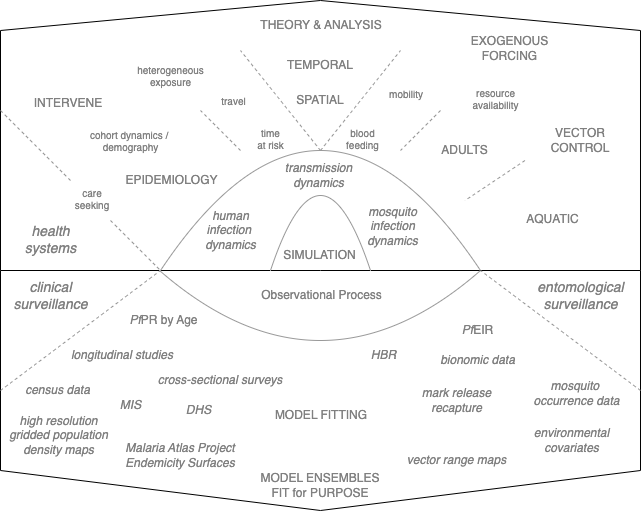
\includegraphics[width=0.8\textwidth,height=\textheight]{../RAMP-Model-Library/Figures/ScalableComplexity.png}
\caption{A schematic diagram of the elements in the framework (top half) and the process of model building and model fitting (bottom half)}
\end{figure}

This book has been written to introduce the features of the framework (see Figure 1.1). The book itself is embedded in the RAMP-Model-Library, which was set up during the primary design phase. The RAMP-Model-Library is where we made all our design mistakes: was the software truly plug-and-play, and was the framework truly extensible? As the primary design phase came to a close, the library that was once the laboratory became a classroom and a museum. The library is being transformed into a resource for any developer who wants to add new base models to the library or add functionality. Most of all, it is being set up for the end user, someone in a malaria program or working with a malaria program who wants to use simulation based analytics to analyze policies. This book is structured into a set of lessons that teach concepts. Some of the concepts build on one another, and others take on new challenges. We combine these lessons into some examples where we show some algorithms to build models fit for purpose. When a topic deserves a deeper dive, we have supplemented this book with vignettes or lessons.

In malaria epidemiology (narrowly defined as a study of infection and disease in humans), the relationship between exposure, infection, immunity, disease, and infectiousness changes in populations as they age, and it is affected by drug taking. This picture grows more complex as we consider intervening with vaccines or monoclonal antibodies, or as we look at interactions with anemia, nutritional status, and human genetics. Our models need to interface with data from clinical settings and research, so they will need to consider diagnostics, parasite counts, detection, and transmission. Combining these factors can give rise to an overwhelming amount of complexity. Later, we will introduce new models and show how it possible to simplify all this complexity and make sense of malaria.

We are interested in using these models to guide policy, which requires both solid computation and good communication. In this book, we lay a foundation for understanding the complexity by studying some simple compartmental models. We will review classical queuing models for superinfection and the multiplicity of infection (MoI); new models for the age of infection (AoI) or stage of infection (SoI); immunity; parasite densities, fever, disease, and detection; gametocytes and transmission, and drug taking. To end up with models that can handle all the complexity, we build probabilistic models that combine these factors. In doing so, we find that we can do some powerful analysis, and we can map the states in these models onto outcomes that matter for research and policy: test positivity, parasite counts, infectiousness, and disease. With patience, we can combine these factors and develop a framework for understanding malaria in populations that match the features of individual-based simulation models. We end up with a sensible understanding malaria epidemiology as ontogeny -- development of immunity as a part of an organisms history. We back this view with some very usable models that capture the changing character of malaria in cohorts of humans as they age.

We are interested in understanding malaria control in context, which requires delving into mosquito ecology and behavior. In this book, we start with a simple model for mosquito ecology and parasite infection dynamics in mosquitoes. We add aquatic population dynamics, mosquito population regulation, and exogenous forcing by weather. Later, we worry about adult mosquito behavioral states such as mating, sugar feeding, and egg laying. We introduce the concept of resource availability, and we develop an understanding of mosquito search and movement in response to resource availability. We take some deep dives to understand how mosquito spatial dynamics work at a fine spatial grain, and then we scale up to understand mosquito populations on landscapes.

At first, we describe mosquito blood feeding and transmission with a few simple parameters. Later, we develop a new model for mosquito blood feeding in a dynamically changing host population with parameters that allow host strata to be more or less available. We also modify our understanding of heterogeneous exposure to biting. We develop a methods for modeling environmental heterogeneity, heterogeneous exposure by age, and a generalized way of handling \href{Frailty}{failty}-- other sources of heterogeneous biting -- through stratification.

We must take a detour to understand how to handle the effects of temperature on the parasite's extrinsic incubation period (EIP). We need a way of dealing with mosquito survival and dispersal through the EIP. This problem has been effectively solved.

To round out this picture, we need a way of dealing with other aspects of human ecology that affect malaria transmission dynamics, including human mobility, human demography, bed net usage, adherance to drugs, and care seeking. Differences among humans call for a synthesis of studies that have identified traits that affect malaria, stratification, and simulation to identify useful ways of propagating the heterogeneity through analyses.

To go along with a theory of transmission, we need a theory of control. We compute effect sizes and evaluate area effects. We develop a generalized concept of effect modification that considers the total effect of a single unit of control. We modify basic processes by including the effects of vector control and mass medical interventions (\emph{e.g.} seasonal malaria chemoprotection, mass drug administration, vaccines, and monoclonal antibodies). Relying on behavioral state models and the concept of resource availability, we develop a models for integrated vector control.

\begin{center}\rule{0.5\linewidth}{0.5pt}\end{center}

In doing all this, we are building on an enormous body of work that started with Ronald Ross. While Ross is better known for identifying malaria parasites in a mosquito gut, which proved that malaria is mosquito transmitted, we are more interested in the academic work that followed.

After winning the Nobel Prize in 1902, Ross was instrumental in building solid quantitative foundations for malaria transmission and its measurement. Ronald Ross wrote the first models describing malaria transmission. In his writings from 1899 to 1908, it's clear that he was searching for quantitative way of saying something simple -- if there are not enough mosquitoes, the malaria transmission can't be sustained. There must be a critical mosquito density, above the cutoff malaria transmission would be sustained, and below it malaria would be eliminated. Ross was looking for a formula that encapsulated his intuition: how were thresholds related to the fact that it took two bites for a mosquito to complete its life cycle? Eventually, Ross wrote down some systems of equations that would describe malaria. The ideas, mathematics, and identification of parameters and processes were extended by other scientists later, most notably Alfred Lotka and George Macdonald.

It seems that the challenge of malaria control was what pushed Ross toward modeling. Ross's first model was a discussion of adult mosquito movement to guide larval source management {[}\protect\hyperlink{ref-RossR1905LogicalBasis}{2}{]}. The first model describing malaria transmission appeared in a book, \emph{The Prevention of Malaria in Mauritius} {[}\protect\hyperlink{ref-RossR1908ReportPrevention}{3}{]}. When it came to thinking through control, Ross found it useful to do the math.

\begin{center}\rule{0.5\linewidth}{0.5pt}\end{center}

This is a book about how to do the math that is required for malaria programs. The goal is to use all the data available, but especially the data generated by malaria programs, to paint a clear picture of malaria transmission as a changing baseline that has been modified by control. The software is structured into three major domains: the humans and malaria epidemiology, including the effects of treating malaria with drugs; the mosquitoes and the way they have been changed by weather and vector control; and parasite transmission through mosquito blood feeding. Within each domain, there are multiple sub-domains, and there are built in design features to deal with heterogeneity and other features for malaria control. After a 140 years of studying malaria, there's a lot of detail that could be important in some way. Part of what we need to do is sort through all that detail to find what is most relevant.

We have organized the concepts in this book around a narrative that allows us to introduce the core concepts -- those that make modular computation possible -- in an order that minimizes the need to draw on unfamiliar concepts. We start with the Ross-Maconald model, but our next task is to update the model for mosquito blood feeding.

Our philosophy has been to design a framework for model building that can be used by programs. The material in this book is designed to be used by non-experts too, so in this context, \emph{model building} means applying a set of tools to to computational tasks we wish our brains could do.

The software we have developed is meant to lower the costs of building and using models. We want programs to be focused on the decisions, the data, the concepts, and the analysis. As a metaphor, some students learn a numerical method for approximating \(\sqrt{2}\) in school, but after learning it once, they stop worrying about \emph{how} it is computed and they punch buttons into a calculator. Knowing how to compute something is sometimes useful, but worrying about how to compute it each time would interrupt the process that called for computing it. Instead, we punch the formula into a scientific calculator or any software that does computation confident that the machine knows how to do it. In applying models, the same kind of logic applies. People need to understand the concepts, but like a calculator, the tools should hide the technical details that don't add to a discussion. The software we have developed is a reliable interface for calculations designed to support policy.

To learn how to use that software, we need to get through a lot of material. The background material in the following presentation is fairly sparse. We are trying to introduce just \emph{enough} mathematics to teach users the critical concepts so they know what the software can do. We assume that the work will be done by teams that include a few people who understand the mathematics, who can guide others through the process. To fill in some of the gaps and technical, we have written (or can write) vignettes. On occasion, the text includes links to these vignettes for those who might find them useful. Please send suggestions about new vignettes to \href{mailto:smitdave@gmail.com}{\nolinkurl{smitdave@gmail.com}}.

The first model we present is a Ross-Macdonald model.

\hypertarget{part-basic-concepts}{%
\part{Basic Concepts}\label{part-basic-concepts}}

\hypertarget{malaria-population-dynamics}{%
\chapter{Malaria Population Dynamics}\label{malaria-population-dynamics}}

We start by introducing a Ross-Macdonald model {[}\protect\hyperlink{ref-SmithDL2012_RossMacdonald}{4}{]}.
This particular system of delay differential equations traces back to a 1982 book chapter written by Joan Aron and Robert May {[}\protect\hyperlink{ref-AronJL1982PopulationDynamics}{5}{]}. We think it's a good starting point.

We chose it because it is \emph{extensible}. The variables in this model represent population densities. The variables are used to compute statistics like \emph{prevalence,} a proportion. The variables in most other versions of the Ross-Macdonald are proportions. In building models, we would sometimes like to change the \emph{total} number of hosts (\emph{i.e.} the denominators), but if the variables in equations described proportions, they are much more difficult to modify.

We chose it because we can bypass a lengthy discussion of the limitations of the Ross-Macdonald model, as it was presented by Macdonald. While Macdonald's analysis and formulas are familiar, they overlooked the role of mosquito ecology. This model lets us bypass a lengthy discussion about history and the way it skews opinions. Our formula for vectorial capacity is consistent with the original, but our analysis includes effects on mosquito ecology.

We chose it because it is \emph{realistic.} Most Ross-Macdonald equations are \emph{autonomous} (time is never used in computing derivatives), but these equations are already non-autonomous (\emph{i.e.} time drives a seasonal pattern). We know that malaria transmission dynamics are forced by exogenous variables (\emph{e.g.}, weather), so why start by avoiding that fact?

We recommend that everyone reads this chapter, even those who are familiar with the Ross-Macdonald model. In writing the equations, we introduced some concepts and conventions that became important for the software design.

\hypertarget{aron-and-mays-equations}{%
\section{Aron and May's Equations}\label{aron-and-mays-equations}}

The simplest quantitative description of malaria dynamics tracks the number of infected and infectious mosquitoes and the number of infected and infectious humans. To develop systems of equations, we assign names to variables that represent these quantities: the number of infected and infectious people is denoted \(X(t)\) (out of \(H\) total); the number of mosquitoes is \(M(t)\); the number of infected mosquitoes is \(Y(t)\) (out of \(M(t)\) total); and the number of infectious mosquitoes is denoted \(Z(t)\) (out of \(M(t)\) total).

In dynamical systems, we ask how the variables (\emph{i.e.} \(M\), \(Y\), \(Z\), and \(X\)) change over time. For our first equation, we start with adult, female mosquito populations. (It is tiresome to repeat \emph{adult, female} each time, and we're ignoring male mosquitoes at this point anyway, so \emph{mosquito} hereafter means \emph{adult, female mosquito}, unless we say otherwise.) The number of mosquitoes is changing as new adults emerge from aquatic habitats or die.

\hypertarget{mosquito-ecology}{%
\subsection{Mosquito Ecology}\label{mosquito-ecology}}

To model changes in \(M\), we assume the following:

\begin{itemize}
\item
  mosquitoes emerge from aquatic habitats at the rate of \(\Lambda(t)\) adults, per day;
\item
  mosquitoes die at a constant rate, \(g\). This is equivalent to assuming that the mosquito lifespan is exponentially distributed with a mean \(1/g\). The fraction surviving one day is \(e^{-g}\).
\end{itemize}

Our first equation describes changes in the number of mosquitoes:

\begin{equation}
\frac{dM}{dt} = \Lambda(t) - g M
\end{equation}

\hypertarget{blood-fed-mosquitoes}{%
\subsection{Blood Fed Mosquitoes}\label{blood-fed-mosquitoes}}

At this point, we will take a detour and define a variable describing the density of mosquitoes that have blood fed at least once, \(V\). After blood feeding, a mosquito is either gravid or \emph{parous}, meaning its ovaries are distended from laying an egg batch. We do this, in part, because the fraction of mosquitoes that are parous is routinely collected, and because it gives us a chance to focus on blood feeding.

To describe \emph{blood feeding}, we assume the following:

\begin{itemize}
\item
  mosquitoes blood feed at the rate \(f\), per mosquito, per day; in this model, this implies that the waiting time to a blood meal is \(1/f\) days.
\item
  a fraction of all mosquito blood meals, \(q\), is taken on humans; we call this the \emph{human fraction}
\item
  the human blood feeding rate is the product of these two parameters, \(fq\), which is defined as the number of human blood meals, per mosquito, per day.
\end{itemize}

The number of human blood meals by a population of vector mosquitoes, per person, per day is called the human biting rate (HBR). In this model, HBR is given by a formula:

\[\mbox{HBR} = \frac{fqM}{H}\]

Later, we discuss the correspondence between the HBR in models and data.

\begin{equation}
\frac{dV}{dt} = f q (M-V) - g V
\end{equation}

We won't use \(V\) to describe the dynamics of infection, but we might find it useful to understand how parity changes in mosquito populations.

\hypertarget{infected-mosquitoes}{%
\subsection{Infected Mosquitoes}\label{infected-mosquitoes}}

Mosquitoes become infected after blood feeding on an infectious human. To model changes in \(Y\), we extend the model of blood feeding to include infection. We need to know what fraction of blood meals end up infecting a mosquito that has not already been infected.

To model changes in \(Y\), we need to describe \emph{infection rates}. We assume the following:

\begin{itemize}
\tightlist
\item
  a fraction of human blood meals, infects mosquitoes. We call this quantity \emph{net infectiousness} (NI) and (for reasons that we will discuss in a moment), we give it a name, \(\kappa\):
\end{itemize}

\[\kappa(t) = c \frac{X(t)}{H}\]

\begin{itemize}
\tightlist
\item
  infected mosquitoes die at the same rate as uninfected mosquitoes.
\end{itemize}

We can now write down our second equation describing changes in the number of infected mosquitoes:

\begin{equation}
\frac{dY}{dt} = f q \kappa (M-Y) -g Y
\end{equation}

\hypertarget{infectious-mosquitoes}{%
\subsection{Infectious Mosquitoes}\label{infectious-mosquitoes}}

To become infectious, a mosquito has to become infected and then survive through the extrinsic incubation period (EIP). We assume:

\begin{itemize}
\item
  mosquitoes become infectious after a fixed delay, \(\tau\) days, called the EIP. The fraction of mosquitoes that survive through the EIP is \(e^{-g \tau}\).
\item
  infectious mosquitoes die at the same rate as other mosquitoes.
\end{itemize}

For a mosquito to become infectious, it must have become infected \(\tau\) days ago and survived through \(\tau\) days with probability \(e^{-g\tau}\). To write this in equations, we use a subscripted \(\tau\) to denote the value of a variable (\(M\), \(Y\) or \(X\)) or term (\(\kappa\)) at time \(t-\tau\). For example \(X_\tau\) is the number of people who were infected and infecious at time \(t-\tau\), and \(M_\tau\) is the number of mosquitoes at time \(t-\tau\).

The number of infectious mosquitoes that are added to the population at a point in time includes all the mosquitoes that became infected at time \(t-\tau\) and survived the EIP. This is our third equation describing changes in the number of infectious mosquitoes:

\begin{equation}
\frac{dZ}{dt} = f q  \kappa_\tau (M_\tau-Y_\tau) e^{-g\tau} -g Z
\end{equation}

Here, \(Z\) represents the number of mosquitoes with \emph{sporozoites} in their salivary glands. The \emph{fraction} of mosquitoes with sporozoites in their salivary glands has been called the \emph{sporozoite rate} (SR), which in our notation is

\[ z = \frac{Z}{M}\]

The number of bites by vector mosquitoes, per person, per day is called the entomological inoculation rate (EIR). It is defined as the product of the HBR and the SR:

\[\mbox{EIR} = \mbox{SR} \times \mbox{HBR}\]

In our notation, the EIR is:

\[\mbox{EIR} = z \frac{fqM}{H} = \frac{fqZ}{H}\]
As with the HBR, we would like to know how to connect estiamted values of the EIR to our formulas. Since that's \emph{really} complicated, we've spent a lot of time in the following sections discussing it.

\hypertarget{RossEqn}{%
\subsection{Infected Humans}\label{RossEqn}}

Humans become infected after being bitten by an infectious mosquito. We assume the following:

\begin{itemize}
\item
  A fraction \(b\) of all bites by infectious mosquitoes cause an infection.
\item
  The hazard rate for infection, also called the \emph{force of infection} (FoI) and denoted \(h\) is \(b \times\) EIR: \[h = fqb \frac{Z}{H}\]
\item
  Infections clear at the rate \(r\), per infection, per day (the average time to clear is \(1/r\) days), and after clearing an infection a person becomes susceptible to infection again.
\end{itemize}

We can now write down our fourth equation describing changes in the number of infected humans:

\begin{equation}
\frac{dX}{dt} = h (H-X) - r X 
\end{equation}

\hypertarget{as-a-system}{%
\subsection{\ldots as a System}\label{as-a-system}}

While we presented these equations one at a time, they work as a system. To see it all at once, we write it here as a system with four equations and two terms:

\begin{equation}
\begin{array}{rl}
\frac{dM}{dt} &= \Lambda(t) - g M \\
\frac{dY}{dt} &= fq\kappa(M-Y) - g Y \\
\frac{dZ}{dt} &= fq\kappa_\tau(M_\tau-Y_\tau)e^{-g\tau} - g Z \\
\frac{dX}{dt} &= h (H-X) - rX  \\ \\ \hline \\ 
\kappa &= c \frac{X(t)}{H} \\
h &= b fq \frac{Z(t)}{H} \\
\end{array}
\end{equation}

\begin{figure}
\centering
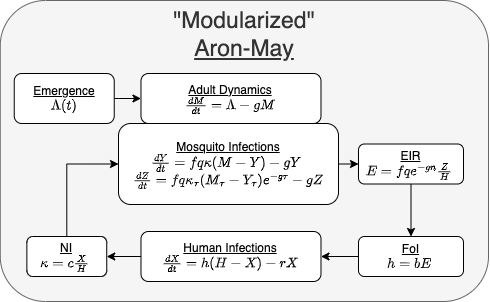
\includegraphics{../RAMP-Model-Library/Figures/AronMay.png}
\caption{A diagram of the a version of the Ross-Macdonald model, using equations from Aron and May {[}\protect\hyperlink{ref-AronJL1982PopulationDynamics}{5}{]}}
\end{figure}

These equations describe processes in three domains (Figure 2.1):

\begin{itemize}
\item
  adult mosquito ecology (\(M\), and perhaps \(V\));
\item
  parasite infection dynamics in mosquito populations (\(Y\) and \(Z\));
\item
  parasite infection dynamics in human populations (\(X\)).
\end{itemize}

The equations describing parasite infections in mosquito populations also include the variable \(M\), so the mosquito infection dynamics are coupled to the mosquito population dynamics. The way we've written the equations, each compartment has an input term (\emph{i.e.}, \(\Lambda\), \(\kappa\), or \(h\)) that depends on something else. We've passed \(\Lambda\) as a parameter. For the infection dynamics, the terms \(\kappa\) and \(h\) couple two separate systems. For adult mosquito dynamics, emergence is passed to the model as a parameters.

There are, of course, more compact ways of writing these equations. We have written the equations this way to emphasize a few things. First, the terms make it clear exactly how the equations in one domain are connected to another. Second, if we wanted to start \emph{changing} some of the assumptions, these terms help to isolate the parts we might like to change. By writing the equations in this modularized form, we can start to understand how we might be able to write software that would allow us to represent mosquito infection dynamics with different systems of equations.

The next step is to find solutions.

\hypertarget{solutions}{%
\section{Solutions}\label{solutions}}

What does a \textbf{solution} to these equations look like?

Solutions to these equations are values of the variables over time \(\left( M(t), Y(t), Z(t), X(t) \right)\) that satisfy the system of four equations described above. We call these solutions \emph{orbits.} To put it another way, if we took the derivatives of the orbits for any variable at any point in time using the basic definition \[\lim_{h\rightarrow 0} \frac{x(t+h)-x(t)}{h},\] and then we used the values of the variables at time \(t\) to compute \(dM/dt\), \(dY/dt\), \(dZ/dt\), and \(dX/dt\) (\emph{i.e.}, using the formulas on the previous page), we would get the same values.

It is important that these orbits are unique: after specifying the \emph{initial values} of the variables, there is one and only one set of orbits that solves the equations. When we solve the equations, we usually produce solutions from a starting point into a future, but the orbits are defined for all time -- \(i.e.\) the process implies the existence of solutions far back into the past. These are deterministic equations, after all.

As written, the equations do not define a \emph{model.} Instead, the equations define a process or a \textbf{model family.} A model is something that \emph{can} produce orbits. A model is defined only after assigning specific values to the parameters. Informally, we will often slip and use the ``model'' to describe a model family. It's easy to slip up, and sometimes we can get by with being sloppy, but we need to remember the distinction. When we say that the software is \emph{modular,} we mean that it is easy to swap out one \emph{model family} for another.

To find solutions of equations we use an R software package called \texttt{deSolve.} Because of the delay for the EIP, these are called \emph{delay differential equations,} which are handled using a function called \texttt{dede}. An important step in solving delay differential equations is a function \texttt{lagvalue()} that computes and returns the values of variables at a time lag, \(\ell\). In these equations, the lag is set by the EIP, \(\tau\), so we must evaluate
\texttt{lagvalue(t-tau).}

In solving \emph{ordinary differential equations,} we must pass initial conditions. To solve a delay differential equations, we must specify the initial conditions for the interval \([-\ell, t_0)\), where \(t_0\) is the point in time when we start computing solutions.
In these equations, since the equation for \(dZ/dt\) looks back \(\tau\) units, we must specify values of \(M(t)\), \(Y(t)\), and \(X(t)\) for all values of \(t \in [-\tau, t_0)\). This forces an awkward choice, since we don't know the solutions backwards in time, but would need to know those solutions to use them. What is typically done -- and we've done it here -- is to specify a constant set of initial values and moving on.

Doing this introduces a little \emph{numerical slop.} By slop, we mean that these values are \emph{not} what we would get if we ran the equations backwards in time. In these equations, it won't affect our analysis most of the time, so we're happy to acknowledge this little problem and find ways around it. It's a little thing, but we should never forget it, because we might find that it \emph{is} affecting our analysis at some point.

With \texttt{deSolve,} solving differential equations is not difficult -- it just involves following a few steps. In the following, we walk through these steps:

\begin{itemize}
\item
  Write a function that computes the derivatives;
\item
  Define initial conditions;
\item
  Define the values of the parameters;
\item
  Define a mesh on time;
\item
  Call a function that solves the equations, such as \texttt{dede} for delay differential equations.
\end{itemize}

Many users will find that reading this code is like learning how to compute \(\sqrt{2}\). If so, feel free to learn it once and then skip it.

\hypertarget{derivatives}{%
\subsection{Derivatives}\label{derivatives}}

The first step is to write down the equations to compute the derivatives. The solver expects a function with three required arguments (in this order):

\begin{itemize}
\item
  \texttt{t} is time
\item
  \texttt{y} is the list of variables
\item
  \texttt{params} is a set of parameters
\end{itemize}

The derivatives are computed and returned in the same order as `y' in a \texttt{list}. To make code that is easy to read, we make \texttt{params} as a \texttt{list} with parameter names (see below), so that inside the function \texttt{with(params,\{...\})}, the parameter names are visible.

\begin{Shaded}
\begin{Highlighting}[]
\NormalTok{dAronMay }\OtherTok{=} \ControlFlowTok{function}\NormalTok{(t, y, params)\{}\FunctionTok{with}\NormalTok{(params,\{}
 
  \CommentTok{\# Variables  }
  \ControlFlowTok{if}\NormalTok{(t}\SpecialCharTok{\textless{}=}\NormalTok{tau) ylag}\OtherTok{\textless{}{-}}\NormalTok{y0 }\ControlFlowTok{else}\NormalTok{ ylag }\OtherTok{\textless{}{-}} \FunctionTok{lagvalue}\NormalTok{(t}\SpecialCharTok{{-}}\NormalTok{tau)}
\NormalTok{  M}\OtherTok{=}\NormalTok{y[}\DecValTok{1}\NormalTok{]; M\_tau }\OtherTok{=}\NormalTok{ ylag[}\DecValTok{1}\NormalTok{]}
\NormalTok{  Y}\OtherTok{=}\NormalTok{y[}\DecValTok{2}\NormalTok{]; Y\_tau }\OtherTok{=}\NormalTok{ ylag[}\DecValTok{2}\NormalTok{]; }
\NormalTok{  Z}\OtherTok{=}\NormalTok{y[}\DecValTok{3}\NormalTok{]; }
\NormalTok{  X}\OtherTok{=}\NormalTok{y[}\DecValTok{4}\NormalTok{]; X\_tau }\OtherTok{=}\NormalTok{ ylag[}\DecValTok{4}\NormalTok{]}
   
  \CommentTok{\# Terms }
\NormalTok{  kappa }\OtherTok{=}\NormalTok{ c}\SpecialCharTok{*}\NormalTok{X}\SpecialCharTok{/}\NormalTok{H; kappa\_tau }\OtherTok{=}\NormalTok{ c}\SpecialCharTok{*}\NormalTok{X\_tau}\SpecialCharTok{/}\NormalTok{H}
\NormalTok{  h }\OtherTok{=}\NormalTok{ b}\SpecialCharTok{*}\NormalTok{f}\SpecialCharTok{*}\NormalTok{q}\SpecialCharTok{*}\NormalTok{Z}\SpecialCharTok{/}\NormalTok{H }
   
  \CommentTok{\# Dynamics }
\NormalTok{  dM }\OtherTok{=} \FunctionTok{Lambda}\NormalTok{(t) }\SpecialCharTok{{-}}\NormalTok{ g}\SpecialCharTok{*}\NormalTok{M}
\NormalTok{  dY }\OtherTok{=}\NormalTok{ f}\SpecialCharTok{*}\NormalTok{q}\SpecialCharTok{*}\NormalTok{kappa}\SpecialCharTok{*}\NormalTok{(M}\SpecialCharTok{{-}}\NormalTok{Y) }\SpecialCharTok{{-}}\NormalTok{g}\SpecialCharTok{*}\NormalTok{Y}
\NormalTok{  dZ }\OtherTok{=}\NormalTok{ f}\SpecialCharTok{*}\NormalTok{q}\SpecialCharTok{*}\NormalTok{kappa\_tau}\SpecialCharTok{*}\NormalTok{(M\_tau}\SpecialCharTok{{-}}\NormalTok{Y\_tau)}\SpecialCharTok{*}\FunctionTok{exp}\NormalTok{(}\SpecialCharTok{{-}}\NormalTok{g}\SpecialCharTok{*}\NormalTok{tau) }\SpecialCharTok{{-}}\NormalTok{g}\SpecialCharTok{*}\NormalTok{Z}
\NormalTok{  dX }\OtherTok{=}\NormalTok{ h}\SpecialCharTok{*}\NormalTok{(H}\SpecialCharTok{{-}}\NormalTok{X)}\SpecialCharTok{{-}}\NormalTok{r}\SpecialCharTok{*}\NormalTok{X}
  
  \FunctionTok{return}\NormalTok{(}\FunctionTok{list}\NormalTok{(}\FunctionTok{c}\NormalTok{(dM, dY, dZ, dX)))}
\NormalTok{\})\} }
\end{Highlighting}
\end{Shaded}

\hypertarget{initial-values}{%
\subsection{Initial Values}\label{initial-values}}

To run the model, we must supply initial values. If you were writing code yourself, it would be important to remember that the initial values and the return value for the derivatives must occur in the same order.

A useful convention in \{R\} is to pass the initial values as a named list. Later, we can turn the outputs into a data frame, and then we can retrieve the variables by name.

\begin{Shaded}
\begin{Highlighting}[]
\NormalTok{y0}\OtherTok{=} \FunctionTok{c}\NormalTok{(}\AttributeTok{M=}\DecValTok{60}\NormalTok{, }\AttributeTok{Y=}\DecValTok{0}\NormalTok{, }\AttributeTok{Z=}\DecValTok{0}\NormalTok{, }\AttributeTok{X=}\DecValTok{1}\NormalTok{)}
\end{Highlighting}
\end{Shaded}

The object \texttt{y0} is a named list -- the names are attached but invisible.

\begin{Shaded}
\begin{Highlighting}[]
\NormalTok{y0}
\end{Highlighting}
\end{Shaded}

\begin{verbatim}
##  M  Y  Z  X 
## 60  0  0  1
\end{verbatim}

When we turn it into a list, with \texttt{as.list,} the names are attached to the values:

\begin{Shaded}
\begin{Highlighting}[]
\FunctionTok{as.list}\NormalTok{(y0)}\SpecialCharTok{$}\NormalTok{M}
\end{Highlighting}
\end{Shaded}

\begin{verbatim}
## [1] 60
\end{verbatim}

If we use \texttt{with}, we create an environment where we can simply use the names:

\begin{Shaded}
\begin{Highlighting}[]
\FunctionTok{with}\NormalTok{(}\FunctionTok{as.list}\NormalTok{(y0), \{}
\NormalTok{  M}
\NormalTok{\})}
\end{Highlighting}
\end{Shaded}

\begin{verbatim}
## [1] 60
\end{verbatim}

\hypertarget{parameter-values}{%
\subsection{Parameter Values}\label{parameter-values}}

We pass the parameters as a list. It might seem like overkill, but we have written a function \texttt{makeParams()} that takes default values and generates a list. This makes it easy to generate a new set of parameter values with alternative values, and it also helps us to write and pass function \(\Lambda(t)\) with parameters we like. By passing the parameter as a list, the parameter values are available to the function \texttt{dAronMay} when we use \texttt{with(params,\ \{\})}.

Note that we have also attached the initial values of the variables as a parameter set, which are the return values for \texttt{lagvalue(t)} when \texttt{t\textless{}0}.

\begin{Shaded}
\begin{Highlighting}[]
\NormalTok{makeParams }\OtherTok{=} \ControlFlowTok{function}\NormalTok{(y0, }
                      \AttributeTok{g=}\DecValTok{1}\SpecialCharTok{/}\DecValTok{12}\NormalTok{, }\AttributeTok{f=}\DecValTok{1}\SpecialCharTok{/}\FloatTok{2.5}\NormalTok{, }\AttributeTok{q=}\FloatTok{0.95}\NormalTok{,  }
                      \AttributeTok{c=}\FloatTok{0.15}\NormalTok{,}
                      \AttributeTok{b=}\FloatTok{0.55}\NormalTok{, }\AttributeTok{r=}\DecValTok{1}\SpecialCharTok{/}\DecValTok{200}\NormalTok{, }\AttributeTok{H=}\DecValTok{1000}\NormalTok{,  }
                      \AttributeTok{m=}\NormalTok{.}\DecValTok{05}\NormalTok{, }\AttributeTok{ss=}\DecValTok{1}\NormalTok{,  }
                      \AttributeTok{tau=}\DecValTok{10}  
\NormalTok{                      )\{}
\NormalTok{  ss }\OtherTok{=} \FunctionTok{min}\NormalTok{(}\DecValTok{1}\NormalTok{,}\FunctionTok{max}\NormalTok{(}\DecValTok{0}\NormalTok{, ss))}
\FunctionTok{return}\NormalTok{(}\FunctionTok{list}\NormalTok{(}\AttributeTok{y0=}\NormalTok{y0,}\AttributeTok{g=}\NormalTok{g,}\AttributeTok{f=}\NormalTok{f,}\AttributeTok{q=}\NormalTok{q,}\AttributeTok{c=}\NormalTok{c,}\AttributeTok{H=}\NormalTok{H,}\AttributeTok{tau=}\NormalTok{tau,}\AttributeTok{b=}\NormalTok{b,}\AttributeTok{r=}\NormalTok{r,}
  \AttributeTok{Lambda =} \ControlFlowTok{function}\NormalTok{(t)\{m}\SpecialCharTok{*}\NormalTok{H}\SpecialCharTok{*}\NormalTok{(}\DecValTok{1} \SpecialCharTok{+}\NormalTok{ ss}\SpecialCharTok{*}\FunctionTok{sin}\NormalTok{(}\DecValTok{2}\SpecialCharTok{*}\NormalTok{pi}\SpecialCharTok{*}\NormalTok{t}\SpecialCharTok{/}\DecValTok{365}\NormalTok{))\})) }
\NormalTok{\} }
\NormalTok{params }\OtherTok{=} \FunctionTok{makeParams}\NormalTok{(y0)}
\end{Highlighting}
\end{Shaded}

To make it absolutely clear, we are assuming:

\begin{itemize}
\item
  \(g=1/12\): mosquitoes live about \(12\) days, on average
\item
  \(f=1/2.5\): mosquitoes feed every 2.5 days, on average
\item
  \(q=0.95\): the human fraction is 95\%; mosquitoes feed on humans 95\% of the time
\item
  \(c=0.15\): about 15\% of bites on infectious humans infect a mosquito
\item
  \(b=0.55\): about 55\% of bites by infective mosquitoes cause an infection
\item
  \(r=1/200\): human infections last about \(200\) days, on average
\item
  \(H=1000\): we're simulating transmission in a population of a thousand humans
\item
  \(\tau=10\): the extrinsic incubation period is about 10 days
\item
  For emergence, we tune the average value using \(m\) and it is scaled to \(H\):

  \begin{itemize}
  \item
    The parameter \(m\) in the function above has been set to \(0.05\) by default.
  \item
    The parameter \(ss\) affects the amplitude of the fluctuations. We force it to take on values between 0 and 1.
  \item
    Emergence is modeled as a sinusoidal function with a yearly cycle.
  \end{itemize}
\end{itemize}

\[\Lambda(t) = m H \left(1 + \sin \left(\frac{2\pi t}{365}\right)\right)\]

\hypertarget{time-mesh}{%
\subsection{Time Mesh}\label{time-mesh}}

We define a mesh over time -- the points in time when we would like to know the values of the variables:

\begin{Shaded}
\begin{Highlighting}[]
\NormalTok{tt }\OtherTok{=} \FunctionTok{seq}\NormalTok{(}\DecValTok{0}\NormalTok{,}\DecValTok{5}\SpecialCharTok{*}\DecValTok{365}\NormalTok{, }\AttributeTok{by=}\DecValTok{5}\NormalTok{) }
\end{Highlighting}
\end{Shaded}

\hypertarget{solving}{%
\subsection{Solving}\label{solving}}

This code solves the equations:

\begin{Shaded}
\begin{Highlighting}[]
\FunctionTok{require}\NormalTok{(deSolve)}
\NormalTok{yout }\OtherTok{\textless{}{-}} \FunctionTok{dede}\NormalTok{(}\AttributeTok{y=}\NormalTok{y0, }\AttributeTok{times=}\NormalTok{tt, }\AttributeTok{func=}\NormalTok{dAronMay, }\AttributeTok{parms=}\NormalTok{params) }
\end{Highlighting}
\end{Shaded}

\hypertarget{visualizing}{%
\subsection{Visualizing}\label{visualizing}}

We write a function so that we can plot things easily:

\begin{Shaded}
\begin{Highlighting}[]
\NormalTok{plotTS\_AronMay }\OtherTok{=} \ControlFlowTok{function}\NormalTok{(yout)\{}\FunctionTok{with}\NormalTok{(}\FunctionTok{data.frame}\NormalTok{(yout),\{}
  \FunctionTok{par}\NormalTok{(}\AttributeTok{mfrow =} \FunctionTok{c}\NormalTok{(}\DecValTok{2}\NormalTok{,}\DecValTok{1}\NormalTok{))}
  \FunctionTok{plot}\NormalTok{(time}\SpecialCharTok{/}\DecValTok{365}\NormalTok{, M, }\AttributeTok{type =} \StringTok{"l"}\NormalTok{, }\AttributeTok{col =} \StringTok{"blue"}\NormalTok{, }
       \AttributeTok{xlab =} \StringTok{"Time (in Years)"}\NormalTok{, }
       \AttributeTok{ylab =} \StringTok{"Mosquito Density"}\NormalTok{, }
       \AttributeTok{main =} \StringTok{"Mosquitoes"}\NormalTok{)}
  \FunctionTok{lines}\NormalTok{(time}\SpecialCharTok{/}\DecValTok{365}\NormalTok{, Y, }\AttributeTok{col =} \StringTok{"purple"}\NormalTok{)}
  \FunctionTok{lines}\NormalTok{(time}\SpecialCharTok{/}\DecValTok{365}\NormalTok{, Z, }\AttributeTok{col =} \StringTok{"red"}\NormalTok{)}
  
  \FunctionTok{plot}\NormalTok{(time}\SpecialCharTok{/}\DecValTok{365}\NormalTok{, X, }\AttributeTok{ylim =} \FunctionTok{c}\NormalTok{(}\DecValTok{0}\NormalTok{,}\DecValTok{1000}\NormalTok{), }\AttributeTok{type =} \StringTok{"l"}\NormalTok{, }
       \AttributeTok{xlab =} \StringTok{"Time (in Years)"}\NormalTok{, }
       \AttributeTok{ylab =} \StringTok{"\# Infected Humans"}\NormalTok{, }
       \AttributeTok{main =} \StringTok{"Humans"}\NormalTok{)}
\NormalTok{\})\}}
\end{Highlighting}
\end{Shaded}

This code plots the outputs:

\begin{Shaded}
\begin{Highlighting}[]
\FunctionTok{plotTS\_AronMay}\NormalTok{(yout)}
\end{Highlighting}
\end{Shaded}

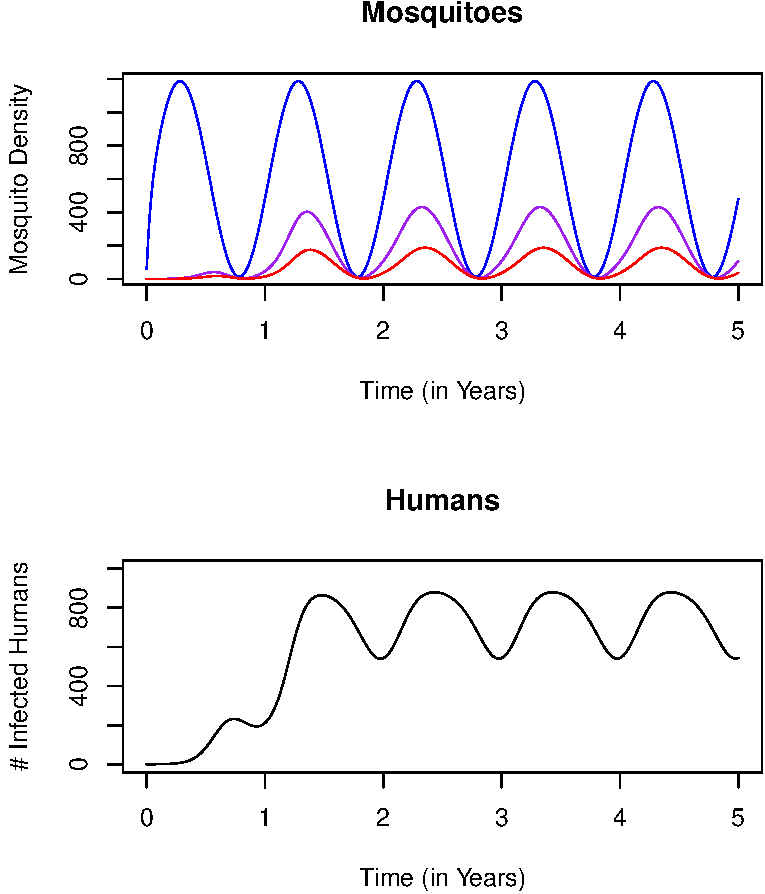
\includegraphics{_main_files/figure-latex/unnamed-chunk-11-1.pdf}

\clearpage

\hypertarget{steady-states}{%
\section{Steady States}\label{steady-states}}

To analyze this system, we first set the parameter \texttt{ss=1}, so that we can look at the system \emph{without} seasonality. Without seasonality, the system is actually \emph{autonomous.} We do this, in part, because the resulting system is easier to understand, which helps us develop intuition that can be applied (albeit with caution) to more complex systems. To be clear, we are dealing with this system:

\begin{equation}
\begin{array}{rl}
\frac{dM}{dt} &= \Lambda - g M \\
\frac{dY}{dt} &= fq\kappa(M-Y) - g Y \\
\frac{dZ}{dt} &= fq\kappa_\tau(M_\tau-Y_\tau)e^{-g\tau} - g Z \\
\frac{dX}{dt} &= h (H-X) - rX  \\ \\ \hline \\ 
\kappa &= c \frac{X(t)}{H} \\
h &= b fq \frac{Z(t)}{H} \\
\end{array}
\end{equation}

\begin{center}\rule{0.5\linewidth}{0.5pt}\end{center}

The first thing to note is that \(M\) affects \(Y\) and \(Z\), which affect \(X\); but \(M\) is not affected by \(Y\) or \(Z\). Mosquito population density is an \emph{exogenous} factor affecting malaria population dynamics.

We can thus treat it separately:

\begin{equation}
\frac{dM}{dt} = \Lambda - g M 
\end{equation}

Since emergence rates are steady, mosquito population density reaches a steady state when \(dM/dt=0\), which occurs at:

\begin{equation}
\bar M = \frac{\Lambda}{g} 
\end{equation}

\begin{center}\rule{0.5\linewidth}{0.5pt}\end{center}

Next, we note that at a steady state, the delayed values of variables and terms don't change, so from \(dY/dt\), we get:

\begin{equation}
g \bar Y = fq\kappa(\bar M- \bar Y) 
\end{equation}

If we substitute the formula for \(\bar M\) and solve for \(\bar Y\), we get:

\begin{equation}
\bar Y = \frac{fq\kappa}{g + fq\kappa} \frac{\Lambda}{g}
\end{equation}

and we substitute the formula for \(g \bar Y\) into \(dZ/dt\) to get:

\begin{equation}
\bar Y e^{-g\tau} = \bar Z
\end{equation}

or equivalently:

\begin{equation}
\bar Z =  \frac{f q \kappa}{g + fq \kappa} \frac{\Lambda}{g} e^{-g\tau} 
\end{equation}

It is a little thing, but the quantity \[S = \frac{fq}{g}\] is the number of bloodmeals a mosquito would take over its lifespan.

At the steady state, \[\mbox{EIR} = fq \frac{\bar Z}{H},\]

but if we rearrange the terms a bit, we get:

\begin{equation}
\mbox{EIR} = fq \frac{\bar Z}{H} = \frac{\Lambda}{H} S^2  e^{-g\tau} \frac{\kappa}{1 + S \kappa} 
\end{equation}

For the moment, we let \[V = \frac{\Lambda}{H} S^2  e^{-g\tau}.\] It is the formula for vectorial capacity. We can thus write:

\begin{equation}
\mbox{EIR} = V \kappa \frac{1}{1 + S \kappa} 
\end{equation}

At the steady state, \[\kappa = c \frac{X}{H}.\] If we substitute this into the expression for the EIR, we get:

\begin{equation}
\mbox{EIR} = c V X\frac{1}{H + c S X} 
\end{equation}

\begin{center}\rule{0.5\linewidth}{0.5pt}\end{center}

Now, we're going to define
\[R_0 = \frac{bcV}{r}.\]

If we plug this into \(dX/dt\) we get an expression that involves only \(X\)

\[\frac{1}{r} \frac{dX}{dt} = X \left( R_0  \frac{H-X}{H + cSX} - 1\right)\]
Since \(X\) is the density of infected humans, it can never be a negative number and it is always smaller than \(H\): we write \(X \in [0, H]\). When \(X\) is very close to \(0\), then

\[\frac{H-X}{H + cSX} \lessapprox 1\]

but in the limit:

\[\lim_{X \rightarrow 0} \frac{H-X}{H + cSX} = 1\]

It follows that when \(X\) is small:

\[\frac{1}{r} \frac{dX}{dt} \approx X \left( R_0  - 1\right)\]
so if \(R_0 >1\), then \(X\) will tend to increase.

We let \[x = \frac{X}{H}\] denote the \emph{prevalence} of infection, or the fraction of people who are infected. Since \(H\) is constant, it is a simple matter to change the variables, and can write:

In this equation, if \(R_0 > 1\), then there is a steady state at:

\[\bar x= \frac{R_0 -1}{R_0 + c S}\]
and if \(R_0<1\), then there is a stable steady state at \(\bar x=0\).

Since at the steady state, \(\kappa = c \bar x\), we can plug this back into the formulas above to get \(\bar Y\) and \(\bar Z\).

What this analysis has shown is that when mosquito population densities are constant, then malaria reaches a steady state: if \(R_0 >1\), then there is a positive endemic equilibrium, and if \(R_0 < 1\), then malaria is absent from the system. The system is said to be stable -- in fact, is is globally asymptotically stable, which means that all the orbits end up converging to the steady state. This statement has been proved many times in many papers, and since this book is focused on policy, we'll let others worry about proofs.

\hypertarget{stable-orbits}{%
\section{Stable Orbits}\label{stable-orbits}}

If emergence rates vary seasonally, how much of the analysis that we did to understand \emph{steady states} still holds? Obviously, things change, but many of the same principles still hold. It is easy enough to simulate, but the resulting dynamics can be quite difficult. Here, we show that the steady state analysis provides a good qualitative guide, but that the answers differ quantitatively.

\hypertarget{orbits}{%
\subsection{Orbits}\label{orbits}}

If \(R_0 >1\), then the system is characterized by \emph{stable orbits} (See Figure 1.1). If \(\Lambda(t)\) has an annual cycle, then after the orbits converge:

\begin{verbatim}
- $M(t+365) = M(t)$; 
- $Y(t+365) = Y(t)$ and $Z(t+365) = Z(t)$; 
- $X(t+365) = X(t)$. 
\end{verbatim}

\begin{figure}
\centering
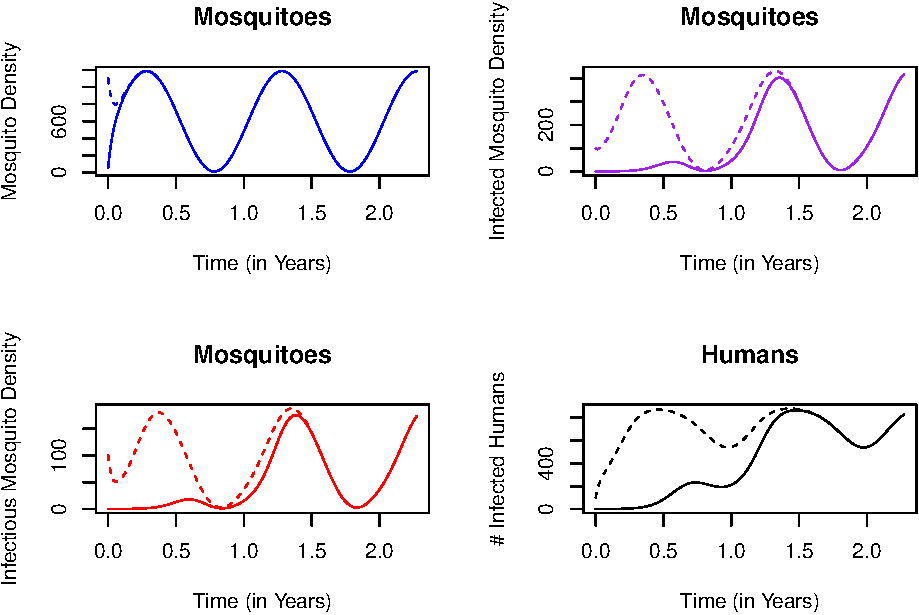
\includegraphics{_main_files/figure-latex/unnamed-chunk-13-1.pdf}
\caption{\label{fig:unnamed-chunk-13}With different initial values, the orbits converge and eventually lie on top of one another.}
\end{figure}

\clearpage

\hypertarget{thresholds}{%
\subsection{Thresholds}\label{thresholds}}

There is a threshold condition \(R_0>1\) that determines whether malaria is endemic, but the formula for \(R_0\) depends on the form of \(\Lambda(t)\). If we set \(R_0=1\), we can show that the threshold for persistence in a seasonal environment is \(R_0 > \sigma > 1\). The math to compute threshold conditions in seasonal environments is in \protect\hyperlink{temporal-dynamics}{Temporal Dynamics}.

\begin{figure}
\centering
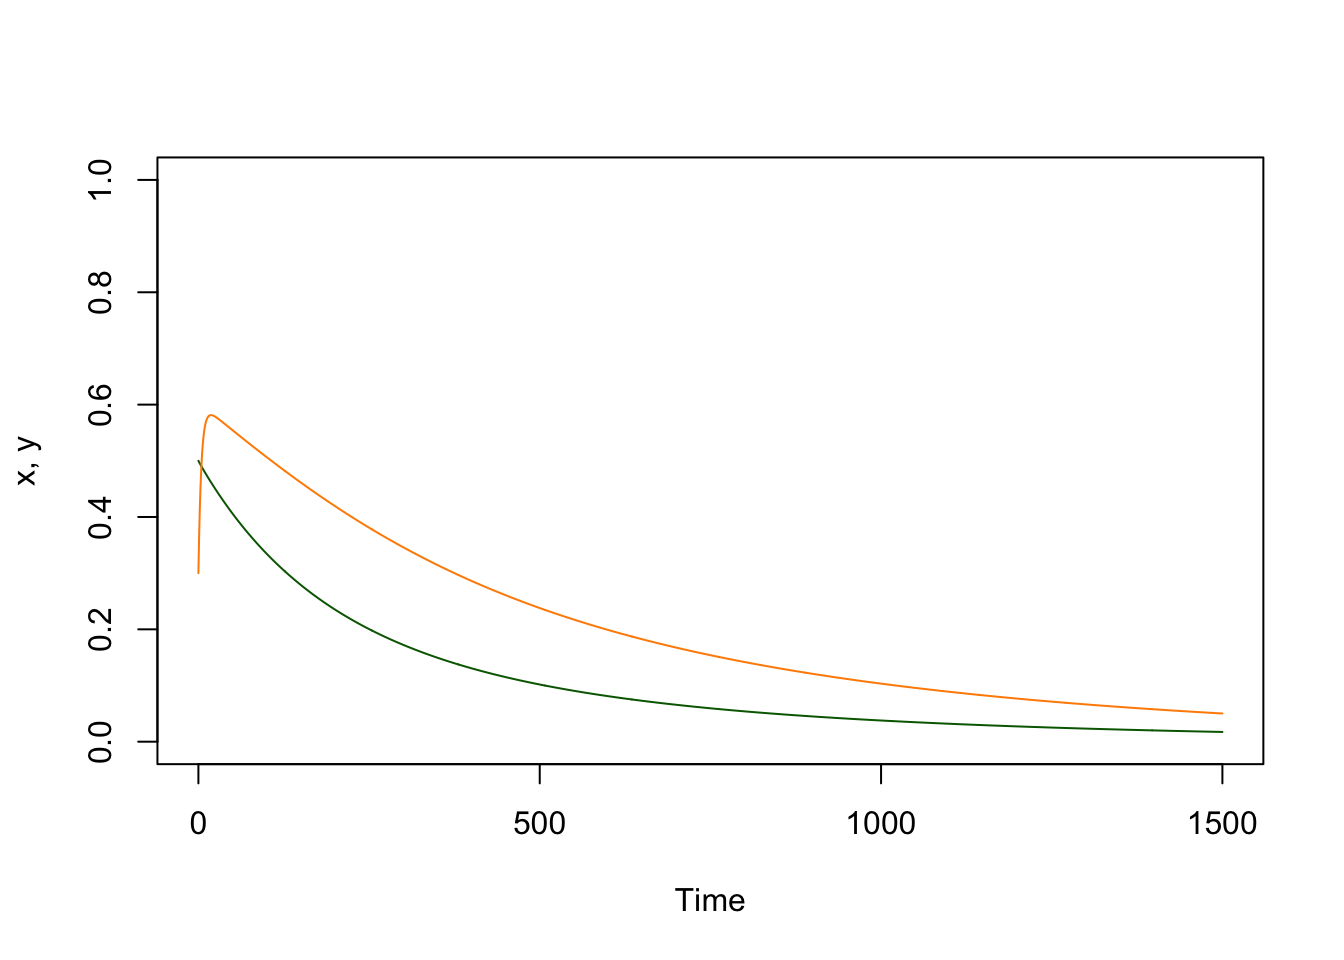
\includegraphics{_main_files/figure-latex/unnamed-chunk-15-1.pdf}
\caption{\label{fig:unnamed-chunk-15}Here, we set \(R_0= 1.02\) for the model with constant emergence, and we show that malaria persists. For the same parameters and for the same \emph{average} emergence rate, malaria declines with seasonality.}
\end{figure}

\clearpage

\hypertarget{average-dynamics}{%
\subsection{Average Dynamics}\label{average-dynamics}}

Away from thresholds, the \emph{average} prevalence of malaria infection is variable in a seasonal environment, though when it has been averaged across the year, it tends to be lower.

\begin{figure}
\centering
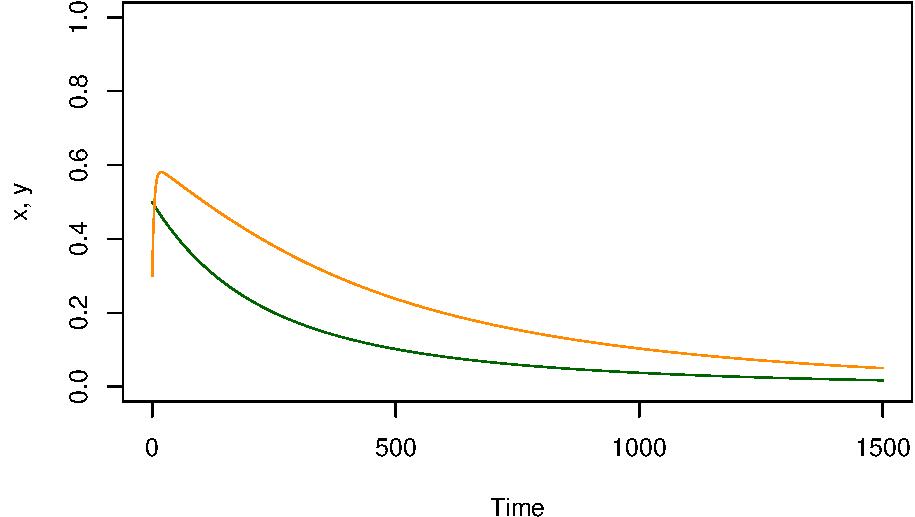
\includegraphics{_main_files/figure-latex/unnamed-chunk-16-1.pdf}
\caption{\label{fig:unnamed-chunk-16}Here, we set \(R_0= 2\) for the model with constant emergence, and we show that the prevalence of malaria is similar in the seasonal environment, but it's higher as transmission peaks, lower in the off-season, and lower overall.}
\end{figure}

\hypertarget{endemic-malaria}{%
\section{Endemic Malaria}\label{endemic-malaria}}

When we do the mathematics, we focus on threshold conditions and the behavior of these systems when malaria is rare. In most places, malaria is endemic so we need to be concerned about malaria immunity and its effects on transmission; malaria is under some level of control; and because of weather and other factors, the baseline conditions change from year to year.

\hypertarget{discussion}{%
\section{Discussion}\label{discussion}}

\hypertarget{mosquito-population-dynamics}{%
\chapter{Mosquito Population Dynamics}\label{mosquito-population-dynamics}}

There are some very good reasons to care about mosquito ecology, particularly when it comes to vector control {[}\protect\hyperlink{ref-BradyOJ2015AdultVector}{6}{]}. In this chapter, we fully define a model for mosquito ecology {[}\protect\hyperlink{ref-SmithDL2013_LarvalDynamics}{7}{]}. The process is actually quite simple:

\begin{itemize}
\item
  We define terms that describe egg-laying by adult mosquitoes;
\item
  We write a basic equation that determines how eggs develop in
  aquatic habitats and then emerge as adults;
\item
  We incorporate seasonality into parameters in an aquatic model;
\item
  We replace the parameter \(\Lambda(t)\) from the Aron-May model with a term that
  describes emergence of adults from aquatic habitats.
\end{itemize}

\hypertarget{aquatic-dynamics}{%
\section{Aquatic Dynamics}\label{aquatic-dynamics}}

\begin{equation}
\begin{array}{rl}
\frac{dL}{dt} &= \eta - (\psi + \phi + \theta L) L \\ 
\frac{dM}{dt} &= \Lambda - g M\\  \\ \hline 
\Lambda &= \frac{\psi L}{2} \\ 
\eta &= \chi \nu M \\ 
\end{array}
\end{equation}

\hypertarget{understanding-mosquito-dynamics}{%
\section{Understanding Mosquito Dynamics}\label{understanding-mosquito-dynamics}}

\hypertarget{measuring-malaria}{%
\chapter{Measuring Malaria}\label{measuring-malaria}}

\hypertarget{realism}{%
\chapter{Realism}\label{realism}}

There are several reasons why models for policy will tend to be more complex than models developed for science. When models are used for policy, the advice should be consistent across studies, which may mean that the models must be complex enough to serve many purposes all at once. To build models that can serve malaria policy, we need the models to be \emph{realistic} enough to be compelling. It might take a lot of work to build a model that resembles malaria in a particular place and time, and it might cut against the instincts we have as scientists to add all that realism, but it's worth it to make the effort if it helps communicate with malaria managers.

In designing a software solution to the problem of building realistic models, we wanted a toolbox to build models that would directly address the concerns of malaria programs. In the chapters that follow, we'll show the features of this framework by constructing examples. If we're principled about it, the primary cost is \emph{computational complexity.} That is something the software was designed to manage. For the moment, we thus want to set aside concerns about \emph{realism} vs.~\emph{abstraction}, about \emph{parsimony}, and about \emph{error propagation,} and we want to simply ask the question of how to build models with the features we want.

This chapter is an overview of the toolbox. We'll cover the same material in much greater detail, with examples, in the chapters that follow.

\hypertarget{stratification}{%
\section{Stratification}\label{stratification}}

The first topic we want to cover is \emph{segmentation} of the human population into \emph{strata.} When we talk about \emph{stratification,} we mean it the narrow sense of segmenting the human population, usually to deal with heterogeneity of some sort.\footnote{In a broader sense, stratification is also about subdividing landscapes into a set of spatial domains that share relevant features in order to \emph{tailor interventions to context.} That is a topic we take up in a separate book,
  ( \textbf{Robust Analytics for Malaria Policy.} ).}
The guiding principle is that our analytics will be more accurate if we identify and remove any sources of heterogeneity, either for estimating the impact of interventions in the past or for projecting those impacts into the future. We acknowledge that models are approximations, and that our approximations don't have to be perfect. The goal is to find ways of propagating uncertainty that are \emph{good enough} for the task at hand.

In malaria epidemiology, \emph{some} kinds of endogenous heterogeneity \emph{could} be built into the \emph{epidemiological state space.} Other kinds of heterogeneity, including consistent differences in exposure, differences in care seeking and drug taking, and differences created by malaria control (\emph{e.g.} net ownership or vaccination), usually require stratification. The decision about how to strike the right balance depends on the model and the purpose of a study.

The framework and supporting software offer a toolbox for stratification. It is designed to stratify populations in a principled way, so that we can \emph{understand} how the heterogeneity affects transmission or outcomes that we care about, but we can also \emph{combine} effects. We want to stratify populations by applying rules that \emph{split} populations when the differences are large enough. (If we started with complex models, we might choose to \emph{join} populations if the differences were small.) By so doing, we can \emph{compare} the behaviors of models that differ from each other in only one way. If the differences are not too large, or if the differences in dynamical behaviors we care about are not too large, we might decide not to split the strata, and use the average. Because of the way models are encoded, it's easy to build models that split the strata in multiple, independent ways.

\hypertarget{strata-in-rosss-model}{%
\subsection{Strata in Ross's model}\label{strata-in-rosss-model}}

As a simple example, consider a simple Ross-style model for infection with exposure and recovery (described in Section \ref{RossEqn}):

\[\frac{dX}{dt} = h (H-X)-r X\]

If exposure is heterogeneous, we could split this population into two strata and add subscripts (\emph{i.e.}, indexed by \(i \in \left\{1,2, \ldots \right\}\)):

\[\frac{dX_i}{dt} =  k_i h (H_i -X_i)-r X_i\]

We hold the \emph{average} FoI constant by constraining the values of \(k_i\):

\[\frac{\sum_i k_i H_i}{H} = 1\]
Stratification is important if the differences are large. With two strata, it would not make sense to stratify if \(k_1 \approx k_2\), but if \(k_2 \gg k_1\) then it might change our expectations, or it might change what we recommend.

\hypertarget{frailties}{%
\subsection{Frailties}\label{frailties}}

We will introduce segmentation first through models of \protect\hyperlink{heterogeneous-exposure}{Heterogeneous Exposure} to malaria, where we consider various sources of \emph{frailty} -- proportional differences in the average hazard rate for infection (\(k_i\), in the example above). These differences in exposure can arise because of age, house type, risky behaviors, other factors. Frailty that is attributable to location (\emph{e.g.} proximity of home to aquatic habitats) can be dealt with by sub-dividing space into \emph{patches,} a topic that is taken up in \protect\hyperlink{space}{Space} below and \protect\hyperlink{spatial-dynamics}{Spatial Dynamics}. Depending on the size of the patches, some differences in average rates of exposure due to location can persist, and these could be dealt with by generic stratification into high \emph{vs.} low exposure strata.

Some of the heterogeneous traits that we care about change dynamically, so we will also need to consider population \emph{flows} among strata, which change the sizes of the strata. We would like to deal with these flows in a principled way. Bed net ownership and use are among the human behaviors that matters most for programs. In some cases, we will want to understand dynamic changes in bed net ownership, the patterns of use among those who own a net, personal protection, and community effects. Later, we show how to construct an example that \emph{describes} all of these aspects of bednets.

Segmentation is what we need to build models of pharmaceutical interventions with waning effectiveness, such as mass vaccination. Among the most important factors in malaria is age. We have defined algorithms to model \protect\hyperlink{aging}{Aging} and other demographic change, the loss of bednets, waning protection or changing housing quality.

\hypertarget{blood-feeding}{%
\section{Blood Feeding}\label{blood-feeding}}

The second topic we must tackle is blood feeding, which is an interaction between mosquitoes and humans. It is an asymmetric relationship -- mosquitoes search for blood hosts, select a host, and blood feed. Humans, for their part, attract mosquitoes from a distance, move around, and spend time in places when mosquitoes are biting. Humans can wear protective clothing (or not), use bed nets (or not), or do other things that make them more or less available to humans. Despite all this, humans are often unaware that they have been bitten.

Transmission occurs during blood feeding, and models of blood feeding \emph{should} be able to take all this heterogeneity into account. If the models do a proper accounting, then the total number of human blood meals taken by mosquitoes would equal the number of blood meals received by humans. In doing so, we find no inspiration from Macdonald, whose description of human blood feeding was simple and phenomenological: a single parameter described the human blood feeding rates. After Garrett-Jones described the human blood index, drawing on decades of work, the one parameter was split into an overall blood feeding rate (\(f\)) and a human fraction (\(q\)). The question left unaddressed by Macdonald was how these rates vary by context, and the consequences for exposure. To do this, we reformulated the algorithm describing blood feeding {[}\protect\hyperlink{ref-WuSL2022SpatialDynamics}{1}{]}.

Over the past two decades, several papers have drawn attention to the way blood feeding behaviors are or ought to be constrained by the availability of vertebrate hosts. It may be fine to assume that the density of vertebrate hosts doesn't change, but \emph{something} should change when a large fraction of people are using bednets. Even with static parameters, we should think through the limiting cases: if there are no vertebrate hosts, then there blood feeding should not occur (\emph{i.e.}, \(f=0\)); if there are no human hosts, then there should be no human blood meals (\(q=0\)); and if there are no alternatives to humans, all blood meals should be on humans (\(q=1\)).

The concepts we devised for blood feeding must, therefore, integrate the notion of frailty with the process of mosquito search. On the one hand, the mosquitoes should blood feed at a slower rate if hosts are unavailable. On the other hand, human biting should become heterogeneous. To arrive at an adequate description, we need to formalize this notion of host availability.
The logic is that mosquitoes \emph{search} for humans. Differences among humans in their attractiveness are represented by a \emph{search weight.} Mosquito search in a place depends on the amount of time spent by humans, but also by daily mosquito activity patterns; from these, we develop a notion of \emph{time at risk} that characterize the way human activities expose them to mosquitoes. The mosquitoes add up all the time at risk spent by all the humans, which gives a measure of their \emph{availability.} Availability describes humans as well as other vertebrate hosts, which are modified by mosquito preferences. The overall feeding rates and the human fraction are computed from availability using \emph{functional responses.}

To complete the picture, we consider how the expected rate of exposure could have a distribution in the population, which we call environmental heterogeneity.

\hypertarget{search-and-risk}{%
\subsection{Search and Risk}\label{search-and-risk}}

\hypertarget{search-weights-and-availability}{%
\subsection{Search Weights and Availability}\label{search-weights-and-availability}}

To deal with heterogeneous exposure and many other phenomena, we need a sensible way of segmenting humans into population \textbf{strata}. Stratification makes it possible to deal with population heterogeneity.

A new model of \textbf{blood feeding} is based on a model of blood feeding as the endpoint of a search for a blood host {[}\protect\hyperlink{ref-WuSL2022SpatialDynamics}{1}{]}.

\begin{itemize}
\item
  Each sub-population has a \emph{search weight} (\(w\)), and the total \emph{availability} of humans for blood feeding (\(W\)) is the sum of the sizes of the strata weighted by their search weights.
\item
  We also consider the availability of alternative vertebrate species for blood feeding (\(O\)).
\end{itemize}

\hypertarget{functional-response}{%
\subsection{Functional Response}\label{functional-response}}

\begin{itemize}
\item
  Mosquito blood feeding rates are computed using a \emph{functional response} to total availability of vertebrate hosts (\(f = F_f(B)\)).
\item
  To compute total availability, we add a scaling parameter on alternative hosts, because mosquito preferences can translate into different patterns of search; total availability is \(B=W + O^\zeta\).
\item
  The human fraction is proportional to the relative availability of hosts \(q = W/B\).
\end{itemize}

\hypertarget{environmental-heterogeneity}{%
\subsection{Environmental Heterogeneity}\label{environmental-heterogeneity}}

\begin{itemize}
\item
  The \emph{search weights} thus translate into a kind of \textbf{\protect\hyperlink{frailty}{Frailty}}, which is one component of \emph{heterogeneous exposure.} Important sources of frailty include bednet use, housing type, and age.
\item
  We also want to consider \emph{variability} in exposure within a stratum -- what is the distribution of the \emph{expected} number of bites over time? We have already discussed frailties, so this is a different kind of heterogeneous exposure that we call \textbf{\protect\hyperlink{environmentalHeterogeneity}{Environmental Heterogeneity}}. This helps us to align models with data: mosquito counts data tend to be described well by \emph{negative binomial} distributions, so it is likely that the distribution of infectious bites also follows a negative binomial distribution. We introduce a function that translate the EIR into the FoI:
  \[h=F_h(E)\]
\end{itemize}

In the Ross-Macdonald model, the underlying assumption is consistent with a Poisson distribution, but we have also derived \emph{negative binomial hazard rates}. Environmental heterogeneity can arise from two sources:

\begin{itemize}
\item
  the aggregated distributions of mosquitoes in micro-habitats, and the redistribution of mosquito populations by wind and weather;
\item
  random movements of humans around mosquito micro-habitats that affect their risk in a way that doesn't tend to change the mean;
\end{itemize}

\hypertarget{mosquito-behavior}{%
\section{Mosquito Behavior}\label{mosquito-behavior}}

\hypertarget{resource-availability}{%
\subsection{Resource Availability}\label{resource-availability}}

\hypertarget{egg-laying}{%
\subsection{Egg Laying}\label{egg-laying}}

\hypertarget{search-and-dispersal}{%
\subsection{Search and Dispersal}\label{search-and-dispersal}}

\hypertarget{space}{%
\section{Space}\label{space}}

Space is big, so we start by drawing boundaries around a part of the world we want to study, that we call the \emph{spatial domain.}

\hypertarget{human-travel-and-mobility}{%
\subsection{Human Travel and Mobility}\label{human-travel-and-mobility}}

The notion of a spatially distributed risk for humans and the modalities of human travel.

\begin{itemize}
\item
  Humans move around, so we develop a model of \emph{time spent}. Time spent is sub-divided into three parts:

  \begin{itemize}
  \item
    time spent at home;
  \item
    time spent traveling, when a night is spent away from home;
  \item
    human mobility, which describes time spent around home when not traveling.
  \end{itemize}
\item
  For travel, we estimate a travel FoI.
\item
  For time at home and mobility, after weighing time spent and mosquito diurnal activity patterns by time of day, we modify time spent to get a notion of \emph{time at risk}
\item
  After modifying time at risk by search weights, mosquito blood meals are distributed among all hosts according to their availability.
\end{itemize}

\hypertarget{mosquito-dispersal-and-demography}{%
\subsection{Mosquito Dispersal and Demography}\label{mosquito-dispersal-and-demography}}

To describe mosquito spatial dynamics, we

\hypertarget{time}{%
\section{Time}\label{time}}

\hypertarget{epidemiology}{%
\section{Epidemiology}\label{epidemiology}}

\hypertarget{aging}{%
\section{Aging}\label{aging}}

Immunity to malaria develops with age and exposure. The development of immunity is probably changing throughout life, so it makes sense to think of malaria epidemiology as ontogeny.

For systems described generically by the state space, \(\mathscr X\), the dynamics we care about have the form:

\[\frac{\partial {\mathscr X}(a,t)}{\partial a} + \frac{\partial {\mathscr X}(a,t)}{\partial t}\]

We might want to deal with malaria differently if we are studying malaria in cohorts. In a population where the FoI over time is \(h(t)\), we might want to follow a birth cohort, so we define \(h_d(a) = h(t-a)\) for all \(t>d\). We can then solve:

\[\frac{d{\mathscr X}}{d a} \]
which produces states in cohorts as they age, \({\mathscr X}(a|h).\)

When we simulate malaria transmission dynamics in populations for policy, we will want to put a mesh on age and segment the population. The dynamics are define for age strata, where the FoI is defined differently for each age stratum:

\[\frac{d{\mathscr X}_a}{d t}\]

which produces age-dependent states over time, \({\mathscr X}_a(t|h).\)

Our algorithms should guarantee that the epidemiological states over time provide an accurate match for the epidemiological states over age.

\hypertarget{mosquito-ecology-1}{%
\section{Mosquito Ecology}\label{mosquito-ecology-1}}

\hypertarget{integrated-vector-control}{%
\section{Integrated Vector Control}\label{integrated-vector-control}}

\hypertarget{pharmaceutic-interventions}{%
\section{Pharmaceutic Interventions}\label{pharmaceutic-interventions}}

\hypertarget{context}{%
\section{Context}\label{context}}

\hypertarget{modularity-and-software}{%
\chapter{Modularity and Software}\label{modularity-and-software}}

Hundreds of publications have described new models of malaria {[}\protect\hyperlink{ref-ReinerRCJ2013SystematicReview}{8},\protect\hyperlink{ref-SmithNR2018AgentbasedModels}{9}{]}. The challenge we have taken on is to find a new way of building models for malaria that draws from all those good ideas to build models at any level of complexity. We want to do this with reusable, professional quality software. Ideally, the models that we develop would be sufficiently complex to address policy questions, yet remain amenable to analysis. To get there, we took a step back to try and understand \emph{malaria models}, and to put this into a birds-eye view of the process of model building.

\begin{center}\rule{0.5\linewidth}{0.5pt}\end{center}

From Ross's first published model in 1905 to the first draft of this book, 117 years have passed. The story of malaria models can be summarized in three epochs.

Ross's models, and contributions to mathematical study of malaria made by Alfred J Lotka (1912-1923), George Macdonald (1950-1968), and Garrett-Jones (1964-1970) take us to the end first epoch, which is marked by the end of the Global Malaria Eradication Programme (GMEP, 1955-1969). As part of the GMEP, Macdonald's formulas were extended by Garrett-Jones into the concept of \emph{vectorial capacity} and a rudimentary theory of vector control. By 1970, the \emph{Ross-Macdonald} model was more than just a set of equations. It was a theory for malaria dynamics and control supported by a well-developed set of concepts, parameters and metrics {[}\protect\hyperlink{ref-SmithDL2012_RossMacdonald}{4}{]}.

Over that same period of time, mathematical theory for directly transmitted diseases took a parallel path, with important mathematical contributions from Kermack and McKendrick, NTJ Bailey, and Bartlett. Sometime around 1980, mathematical epidemiology began a period of innovation and synthesis, particularly after the publications of Robert May and Roy Anderson made it a mainstream activity in departments of ecology.

In malaria and mosquito-borne diseases, Klaus Dietz publications span the second epoch (1971-2006), including development of a mathematical model with immunity for the Garki Project {[}\protect\hyperlink{ref-DietzK1974MalariaModel}{10}{]}, work on the dynamics of malaria under treatment by drugs {[}\protect\hyperlink{ref-DietzK1975ModelsParasitic}{11}{]}, seasonality {[}\protect\hyperlink{ref-DietzK1976IncidenceInfectious}{12}{]}, and heterogeneous biting {[}\protect\hyperlink{ref-DietzK1980ModelsVectorborne}{13},\protect\hyperlink{ref-DietzK1988EpidemiologicalModels}{14}{]}. During this time, theory developed for malaria borrowed concepts and methods. In spatial dynamics, the patch models of Yorke and ** were modified to by Dye and Hasibeder to describe mosquito-borne pathogens {[}\protect\hyperlink{ref-DyeC1986PopulationDynamics}{15},\protect\hyperlink{ref-HasibederG1988PopulationDynamics}{16}{]}.

The last epoch of malaria, which starts around 2006, is marked by two major developments: a maturing theory of malaria control; and the rise of branded, individual-based models.

The publication of \emph{OpenMalaria} in 2006 marks the beginning of the last epoch of malaria. Some important antecedents were Dana Fochs models for \emph{Aedes} dynamics and dengue virus transmission, as \emph{CIMSiM} and \emph{DENSiM}. In malaria, several within-host models had been developed {[}\protect\hyperlink{ref-MolineauxL1999ReviewIntrahost}{17},\protect\hyperlink{ref-MolineauxL2001PlasmodiumFalciparum}{18}{]}. \emph{OpenMalaria} traces its history back to an intrahost model developed by Dietz and Louis Molineaux {[}\protect\hyperlink{ref-MolineauxL2001PlasmodiumFalciparum}{18}{]}. After \emph{OpenMalaria,} two other branded individual-based models were developed. One was developed by a team at Imperial College called \emph{Malaria Tools.} Another was developed by a team at the Institute for Disease Modeling called \emph{eMod.} The fact that the models were named and branded was significant -- the authors had developed software that they would maintain and that they were willing to stand behind. The models had finally dealt with \emph{disease} in a serious way, and through publications, the fitted models demonstrated a fidelity to evidence. The branding signaled continuity and consistency.

Around 2007, new models of vector control began to appear that related intevention coverage levels to effect sizes. Macdonald's work had focused on sensitivity to parameters, and the GMEP emphasized technical efficiency to achieve very high coverage (with IRS). Garrett-Jones developed vectorial capacity as a way of understanding vector control and effect modification by insecticide resistance. The new models extended Garrett-Jones ideas. The need for new models was motivated, at least in part, by the goal of achieving universal coverage with ITNs. What were reasonable coverage targets? The new generation of vector control models introduced the concept of an effect size on transmission as a function of intervention coverage levels, where coverage had one definition for operations (\emph{e.g.} something like ownership) and another for effect sizes (\emph{e.g.} related to vector contact rates with interventions). The goal of achieving very high coverage with ITNs bumped into the reality that nets are not durable, so new models have been devised to look at intervention coverage in relation to distribution schemes and product durability. While these concepts had been considered during the GMEP design phase, they did not appear in Macdonald's models.

\begin{center}\rule{0.5\linewidth}{0.5pt}\end{center}

If we want to take advantage of all the research that has been done, we need a way of understanding malaria models and the whole business of model building.

\hypertarget{model-building}{%
\section{Model Building}\label{model-building}}

Model building is a fairly involved process that includes several unavoidable steps:

\begin{itemize}
\item
  There must be some motivation for building a model, which usually starts with a conversation, boxes and arrows drawn on paper or a chalkboard or whiteboard. The process involves refining the questions, until there's a well-formed idea -- a reason for building a model.
\item
  The idea gets translated into mathematics. The boxes get translated into variables, the arrows are rate parameters, a mathematical formalism is selected.
\item
  The model gets analyzed. In some cases, when the model complexity exceeds a very low threshold on complexity,
  this is done with pencil and paper. It is only possible to analyze individual parts of the model this way.
\item
  The model gets translated into pseudo-code, and then it gets implemented as software that can produce output. This is followed by a long and painful process of verifying that the software does what the pseudo-code says it \emph{should} do. After awhile, the software is trusted, and it's time to use it.
\item
  Some thought is given to the correspondence between the variables in a model, observable quantities, and the observational process itself. This process can be a part of what happens above, but at some point, the models need to be fitted to data.
\item
  The software produces output and then: the outputs are visualized; models are fitted to data; graphs are made; papers or reports are published; and careers advance.
\end{itemize}

That's the simple story of model development. What happens next is could be one of the following:

\begin{itemize}
\item
  Someone re-examines an existing model and notices it is inadequate in some way: it is missing some features, or it might make an assumption that ought to be modified. Simple models become spatial models, single populations are structured.
\item
  Someone decides to implement the model in a different way, perhaps with a different mathematical formalism. Continuous time models are translated into discrete time models. Deterministic models become stochastic. Autonomous processes become non-autonomous.
\end{itemize}

Through this process, hundreds of malaria models were published.

A problem with this process has been that the software is often developed for bespoke tasks (\emph{i.e.} to publish a paper). The software is often poorly documented and difficult to reuse. The costs of building a model for one task limited the complexity of the model. It was difficult to combine elements of one model developed for one purpose, with someone else's model developed for another purpose.

In malaria, this \emph{ad hoc} process of writing new models was found to be inadequate to serve the broad range of policy questions. One way of dealing with the complexity was to build individual-based models, but individual-based models have some of the same limitations as reality.

\hypertarget{modular-computation}{%
\section{Modular Computation}\label{modular-computation}}

Before \emph{OpenMalaria}, most models of malaria modified the Ross-Macdonald model in one way {[}\protect\hyperlink{ref-ReinerRCJ2013SystematicReview}{8}{]}. The innovation was focused on specific themes or questions: how long would an infection last in models with superinfection?

\hypertarget{exde}{%
\subsection{\texorpdfstring{\texttt{exDE}}{exDE}}\label{exde}}

We have written the software that solves these equations in a package called \href{https://cran.r-project.org/web/packages/exDE/index.html}{\texttt{exDE}}.

\hypertarget{part-transmission}{%
\part{Transmission}\label{part-transmission}}

\hypertarget{heterogeneous-exposure}{%
\chapter{Heterogeneous Exposure}\label{heterogeneous-exposure}}

For humans, exposure to malaria means exposure to the bites of infectious mosquitoes. A problem that we'll have to deal with sooner or later is that exposure risk differs among humans over space and time. While this might seem like an odd thing to introduce so early, we will have to tackle the topic sometime. The discussion of {[}Heterogeneous Biting{]}, in the previous chapter, showed that heterogeneity plays an important in understanding transmission and thresholds. This discussion of heterogeneous exposure (\emph{i.e.}, looking at heterogeneous biting from the human side) is a good way of introducing some of the core concepts that are built into the framework:

\begin{itemize}
\item
  {[}Heterogeneous Biting{]} is one way of getting around a conundrum. In models with homogeneous biting, the relationship between \emph{average} mosquito density and the prevalence of infection would lead us to make quantitative predictions about the likely effects of vector control.
\item
  We discuss two different kinds of heterogeneous exposure: frailty, and environmental heterogeneity. In a nutshell, frailty multiplies the mean hazard rate for a sub-population by some amount \(k\). Environmental heterogeneity does not affect the mean, but it changes the distribution of the mean.
\item
  We introduce the idea that we can deal with frailties in human populations by segmenting the population into strata.
\item
  We set the stage for a new model of mosquito \textbf{blood feeding} that we introduce in the next chapter.
\item
  In a chapter on \protect\hyperlink{approximation}{Approximation}, we use these models to discuss the problem of model-based inference.
\end{itemize}

\hypertarget{overview}{%
\section{Overview}\label{overview}}

Some reasons heterogeneous exposure to malaria have been documented in hundreds of studies. This is an overview.

\hypertarget{age}{%
\subsection{Age}\label{age}}

\begin{itemize}
\item
  Port, Boreham
\item
  Carnevale
\end{itemize}

\hypertarget{location}{%
\subsection{Location}\label{location}}

\hypertarget{house-type}{%
\subsection{House Type}\label{house-type}}

\hypertarget{activities}{%
\subsection{Activities}\label{activities}}

\hypertarget{frailty}{%
\section{Frailty}\label{frailty}}

In general, we define frailty as a multiplicative factor on the FoI. If the average FoI in the population is \(h\), then the FoI in a stratum is \(hk\). The size of the stratum, \(p_k\), is constrained such that:

\[\int_0^\infty k \; p_k \; dk = 1\]

With this constraint, the mean FoI in the population is \(h\).

Continuous distributions are difficult to extend, but we can stratify a population to accomplish some of the same effects.

\hypertarget{environmentalHeterogeneity}{%
\section{Environmental Heterogeneity}\label{environmentalHeterogeneity}}

\hypertarget{blood-feeding-1}{%
\chapter{Blood Feeding}\label{blood-feeding-1}}

\hypertarget{availability-and-blood-feeding-rates}{%
\section{Availability and Blood Feeding Rates}\label{availability-and-blood-feeding-rates}}

\hypertarget{host-selection}{%
\section{Host Selection}\label{host-selection}}

\hypertarget{spatial-dynamics}{%
\chapter{Spatial Dynamics}\label{spatial-dynamics}}

\hypertarget{temporal-dynamics}{%
\chapter{Temporal Dynamics}\label{temporal-dynamics}}

\hypertarget{cohort-dynamics}{%
\chapter{Cohort Dynamics}\label{cohort-dynamics}}

We need a way of incorporating age into our models.

\hypertarget{boxcar-models}{%
\section{Boxcar Models}\label{boxcar-models}}

\hypertarget{delay}{%
\section{Delay}\label{delay}}

\hypertarget{demography}{%
\chapter{Demography}\label{demography}}

\hypertarget{migration}{%
\section{Migration}\label{migration}}

\hypertarget{stratification-1}{%
\chapter{Stratification}\label{stratification-1}}

\hypertarget{part-humans}{%
\part{Humans}\label{part-humans}}

\hypertarget{human-behaviors-and-ecology}{%
\chapter{Human Behaviors and Ecology}\label{human-behaviors-and-ecology}}

\hypertarget{human-mobility}{%
\chapter{Human Mobility}\label{human-mobility}}

\hypertarget{human-travel-and-malaria-importation}{%
\chapter{Human Travel and Malaria Importation}\label{human-travel-and-malaria-importation}}

\hypertarget{part-epidemiology}{%
\part{Epidemiology}\label{part-epidemiology}}

\hypertarget{malaria-infection}{%
\chapter{Malaria Infection}\label{malaria-infection}}

In the following sections, we walk through several models for the dynamics of malaria infection and immunity in humans. We cover infection and detection, immunity, infectiousness, disease, drug taking, and cohort dynamics.

\hypertarget{overview-1}{%
\section{Overview}\label{overview-1}}

\hypertarget{multiplicity-of-infection-moi}{%
\section{Multiplicity of Infection (MoI)}\label{multiplicity-of-infection-moi}}

\hypertarget{age-of-infection-aoi}{%
\section{Age of Infection (AoI)}\label{age-of-infection-aoi}}

\hypertarget{stage-of-infection-soi}{%
\section{Stage of Infection (SoI)}\label{stage-of-infection-soi}}

\hypertarget{malaria-immunity}{%
\chapter{Malaria Immunity}\label{malaria-immunity}}

Exposure \emph{vs.} age.

\hypertarget{the-garki-model}{%
\section{The Garki Model}\label{the-garki-model}}

\hypertarget{stage-structured-immunity}{%
\section{Stage-Structured Immunity}\label{stage-structured-immunity}}

\hypertarget{strain-specific-immunity}{%
\section{Strain Specific Immunity}\label{strain-specific-immunity}}

\hypertarget{memory-tracking}{%
\section{Memory Tracking}\label{memory-tracking}}

\hypertarget{age-vs.-prevalence}{%
\section{\texorpdfstring{Age \emph{vs.} Prevalence}{Age vs. Prevalence}}\label{age-vs.-prevalence}}

\hypertarget{detecting-parasites}{%
\chapter{Detecting Parasites}\label{detecting-parasites}}

\hypertarget{parasite-densities-and-detection}{%
\section{Parasite Densities and Detection}\label{parasite-densities-and-detection}}

\hypertarget{light-microscopy}{%
\section{Light Microscopy}\label{light-microscopy}}

\hypertarget{biomarkers-and-rdts}{%
\section{Biomarkers and RDTs}\label{biomarkers-and-rdts}}

\hypertarget{pcr}{%
\section{PCR}\label{pcr}}

\hypertarget{gametocytes-and-infectiousness}{%
\chapter{Gametocytes and Infectiousness}\label{gametocytes-and-infectiousness}}

\hypertarget{gametocytemia}{%
\section{Gametocytemia}\label{gametocytemia}}

\hypertarget{anti-gametocyte-immunity}{%
\section{Anti-Gametocyte Immunity}\label{anti-gametocyte-immunity}}

\hypertarget{fever-and-severe-disease}{%
\chapter{Fever and Severe Disease}\label{fever-and-severe-disease}}

\hypertarget{fever}{%
\section{Fever}\label{fever}}

\hypertarget{anemia}{%
\section{Anemia}\label{anemia}}

\hypertarget{severe-disease}{%
\section{Severe Disease}\label{severe-disease}}

\hypertarget{care-seeking}{%
\chapter{Care Seeking}\label{care-seeking}}

\hypertarget{drug-taking}{%
\chapter{Drug Taking}\label{drug-taking}}

\hypertarget{curing-infections}{%
\section{Curing Infections}\label{curing-infections}}

\hypertarget{chemoprotection}{%
\section{Chemoprotection}\label{chemoprotection}}

\hypertarget{adherance}{%
\section{Adherance}\label{adherance}}

\hypertarget{treatment-rates}{%
\section{Treatment Rates}\label{treatment-rates}}

\hypertarget{pharmaceutical-interventions}{%
\chapter{Pharmaceutical Interventions}\label{pharmaceutical-interventions}}

\hypertarget{smc}{%
\section{SMC}\label{smc}}

\hypertarget{mda}{%
\section{MDA}\label{mda}}

\hypertarget{drugs}{%
\section{Drugs}\label{drugs}}

\hypertarget{vaccines}{%
\section{Vaccines}\label{vaccines}}

\hypertarget{malaria-epidemiology}{%
\chapter{Malaria Epidemiology}\label{malaria-epidemiology}}

\hypertarget{age-of-the-youngest-infection}{%
\section{Age of the Youngest Infection}\label{age-of-the-youngest-infection}}

\hypertarget{part-mosquito-ecology}{%
\part{Mosquito Ecology}\label{part-mosquito-ecology}}

\hypertarget{mosquitoes}{%
\chapter{Mosquitoes}\label{mosquitoes}}

An overview of mosquito ecology,

\hypertarget{behavioral-state-models}{%
\chapter{Behavioral State Models}\label{behavioral-state-models}}

\hypertarget{aquatic-ecology}{%
\chapter{Aquatic Ecology}\label{aquatic-ecology}}

\hypertarget{mosquito-microecology}{%
\chapter{Mosquito Microecology}\label{mosquito-microecology}}

Modeling mosquito population dynamics on point sets.

\hypertarget{mosquito-dispersal}{%
\chapter{Mosquito Dispersal}\label{mosquito-dispersal}}

\hypertarget{microsimulation}{%
\chapter{Microsimulation}\label{microsimulation}}

\hypertarget{mosquito-ecology-2}{%
\chapter{Mosquito Ecology}\label{mosquito-ecology-2}}

\hypertarget{population-dynamics}{%
\section{Population Dynamics}\label{population-dynamics}}

\hypertarget{vector-competence}{%
\chapter{Vector Competence}\label{vector-competence}}

\hypertarget{measuring-mosquitoes}{%
\chapter{Measuring Mosquitoes}\label{measuring-mosquitoes}}

\hypertarget{part-malaria-control}{%
\part{Malaria Control}\label{part-malaria-control}}

\hypertarget{vector-control}{%
\chapter{Vector Control}\label{vector-control}}

Towards a theory of vector control.

\hypertarget{insecticide-treated-bednets}{%
\chapter{Insecticide-Treated Bednets}\label{insecticide-treated-bednets}}

\hypertarget{indoor-residual-spraying}{%
\chapter{Indoor Residual Spraying}\label{indoor-residual-spraying}}

\hypertarget{larval-source-management}{%
\chapter{Larval Source Management}\label{larval-source-management}}

\hypertarget{attractive-toxic-sugar-baits}{%
\chapter{Attractive Toxic Sugar Baits}\label{attractive-toxic-sugar-baits}}

\hypertarget{integrated-vector-control-1}{%
\chapter{Integrated Vector Control}\label{integrated-vector-control-1}}

\hypertarget{spatial-control}{%
\chapter{Spatial Control}\label{spatial-control}}

\hypertarget{pharmaceutical-interventions-1}{%
\chapter{Pharmaceutical Interventions}\label{pharmaceutical-interventions-1}}

\hypertarget{smc-1}{%
\section{SMC}\label{smc-1}}

\hypertarget{mda-1}{%
\section{MDA}\label{mda-1}}

\hypertarget{drugs-1}{%
\section{Drugs}\label{drugs-1}}

\hypertarget{vaccines-1}{%
\section{Vaccines}\label{vaccines-1}}

\hypertarget{spatial-concepts-and-connectivity}{%
\chapter{Spatial Concepts and Connectivity}\label{spatial-concepts-and-connectivity}}

\hypertarget{part-estimation}{%
\part{Estimation}\label{part-estimation}}

\hypertarget{approximation}{%
\chapter{Approximation}\label{approximation}}

In this chapter, we use some of the simple models we've developed to introduce some basic ideas.

\begin{itemize}
\item
  Because it is easy for models of heterogeneous exposure, we introduce a \emph{model to model distance metric} for models that makes it possible to rigorously measure the distance between two models.
\item
  Using distance metrics, we use model-model comparison to show how models approximate each another. Informally, we compare this to a one way \emph{model to data distance metric} that can be used to compare how far two models are from some data set. We imagine an unobserved real world, and we show how information bout the real world is transferred through data.
\end{itemize}

\hypertarget{the-distance-between-two-models}{%
\section{The Distance between Two Models}\label{the-distance-between-two-models}}

\hypertarget{the-distance-from-models-to-data}{%
\section{The Distance from Models to Data}\label{the-distance-from-models-to-data}}

\hypertarget{exposure-and-infection}{%
\chapter{Exposure and Infection}\label{exposure-and-infection}}

The relationships between the annual \emph{Pf}EIR, the \emph{Pf}FoI, and the \emph{Pf}PR are among the most important in malaria. A few studies analyzed the data {[}\protect\hyperlink{ref-BeierJC1999ShortReport}{19},\protect\hyperlink{ref-HaySI2005UrbanizationMalaria}{20}{]}. The first paper I wrote on the topic, in 2005, suggested an important role for heterogeneous biting {[}\protect\hyperlink{ref-SmithDL2005_EIRvPR}{21}{]}. At the time, we were thinking mainly about frailty. After some correspondence, we took a closer look at the relationship between the \emph{Pf}EIR and the \emph{Pf}FoI {[}\protect\hyperlink{ref-SmithDL2010_InefficientTransmission}{22}{]}, which helped us rule out immunity. With some data in hand, we took a closer look at heterogeneous exposure {[}\protect\hyperlink{ref-CooperL2019ParetoRules}{23}{]}, which drew our attention to environmental heterogeneity. Meanwhile, we developed the age-standardization algorithms for the Malaria Atlas Project {[}\protect\hyperlink{ref-SmithDL2007_StandardizingPfPR}{24}{]}. As we grappled with the data from Bioko Island, it became clear that malaria importation could be an important factor {[}\protect\hyperlink{ref-GuerraCA2019HumanMobility}{25}{]}. None of this considered either seasonality or drug taking and chemo-protection.

The \emph{Pf}PR to \emph{Pf}EIR converstion algorthims defined in \ref{pr2eir} are among the most important for policy.

\hypertarget{data}{%
\section{Data}\label{data}}

\hypertarget{eir-vs.-pr}{%
\subsection{EIR vs.~PR}\label{eir-vs.-pr}}

We have revisited the relationship one more time, but we do it in two steps. First, we take another look at the EIR-PR and EIR-FoI data, with a focus on \emph{house effects}

\hypertarget{eir-vs.-foi}{%
\subsection{EIR vs.~FoI}\label{eir-vs.-foi}}

\hypertarget{chemoprotection-1}{%
\subsection{Chemoprotection}\label{chemoprotection-1}}

\hypertarget{models}{%
\section{Models}\label{models}}

Second, we re-evaluate the many sources of variability, and how each one works across the spectrum of transmission:

\begin{itemize}
\item
  Age: What is the age of the population being examined?
\item
  Drug Taking and Chemoprotection: What is the distribution of drug-taking rates and habits in the population?
\item
  Pre-erythrocytic Immunity
\item
  Heterogeneous Exposure

  \begin{itemize}
  \item
    seasonality: how much does seasonality affect the probability of detection?
  \item
    \protect\hyperlink{frailty}{Frailty} (Section \ref{frailty})

    \begin{itemize}
    \item
      age
    \item
      other
    \end{itemize}
  \item
    \protect\hyperlink{environmentalHeterogeneity}{Environmental Heterogeneity} (Section \ref{environmentalHeterogeneity})
  \end{itemize}
\item
  Travel Exposure and Malaria Importation
\item
  Immunity

  \begin{itemize}
  \item
    maternal protection
  \item
    detection
  \end{itemize}
\end{itemize}

\hypertarget{pr2eir}{%
\section{\texorpdfstring{\emph{Pf}PR \(\rightarrow\) \emph{Pf}EIR}{PfPR \textbackslash rightarrow PfEIR}}\label{pr2eir}}

\hypertarget{model-libraries}{%
\chapter{Model Libraries}\label{model-libraries}}

\hypertarget{part-supplements}{%
\part{Supplements}\label{part-supplements}}

\hypertarget{references}{%
\chapter{References}\label{references}}

If you want a PDF and can't find it at the link provided, let us know and we can help you find a copy.

\hypertarget{refs}{}
\begin{CSLReferences}{0}{0}
\leavevmode\vadjust pre{\hypertarget{ref-WuSL2022SpatialDynamics}{}}%
\CSLLeftMargin{1. }%
\CSLRightInline{Wu SL, Henry JM, Citron DT, Mbabazi Ssebuliba D, Nakakawa Nsumba J, Sánchez C. HM, et al. Spatial {Dynamics} of {Malaria Transmission}. 2022. Available: \url{http://medrxiv.org/content/early/2022/11/15/2022.11.07.22282044.abstract}}

\leavevmode\vadjust pre{\hypertarget{ref-RossR1905LogicalBasis}{}}%
\CSLLeftMargin{2. }%
\CSLRightInline{Ross R. The logical basis of the sanitary policy of mosquito reduction. Science. 1905;22: 689--699. doi:\href{https://doi.org/10.1126/science.22.570.689}{10.1126/science.22.570.689}}

\leavevmode\vadjust pre{\hypertarget{ref-RossR1908ReportPrevention}{}}%
\CSLLeftMargin{3. }%
\CSLRightInline{Ross R. Report on the {Prevention} of {Malaria} in {Mauritius}. {London}: {Waterlow}; 1908. Available: \url{https://play.google.com/store/books/details?id=0Mc1AQAAMAAJ}}

\leavevmode\vadjust pre{\hypertarget{ref-SmithDL2012_RossMacdonald}{}}%
\CSLLeftMargin{4. }%
\CSLRightInline{Smith DL, Battle KE, Hay SI, Barker CM, Scott TW, McKenzie FE. Ross, {Macdonald}, and a theory for the dynamics and control of mosquito-transmitted pathogens. PLoS Pathog. 2012;8: e1002588. doi:\href{https://doi.org/10.1371/journal.ppat.1002588}{10.1371/journal.ppat.1002588}}

\leavevmode\vadjust pre{\hypertarget{ref-AronJL1982PopulationDynamics}{}}%
\CSLLeftMargin{5. }%
\CSLRightInline{Aron JL, May RM. The population dynamics of malaria. In: Anderson RM, editor. The {Population Dynamics} of {Infectious Diseases}: {Theory} and {Applications}. {Boston, MA}: {Springer US}; 1982. pp. 139--179. doi:\href{https://doi.org/10.1007/978-1-4899-2901-3_5}{10.1007/978-1-4899-2901-3\_5}}

\leavevmode\vadjust pre{\hypertarget{ref-BradyOJ2015AdultVector}{}}%
\CSLLeftMargin{6. }%
\CSLRightInline{Brady OJ, Godfray HCJ, Tatem AJ, Gething PW, Cohen JM, McKenzie FE, et al. Adult vector control, mosquito ecology and malaria transmission. Int Health. 2015;7: 121--129. doi:\href{https://doi.org/10.1093/inthealth/ihv010}{10.1093/inthealth/ihv010}}

\leavevmode\vadjust pre{\hypertarget{ref-SmithDL2013_LarvalDynamics}{}}%
\CSLLeftMargin{7. }%
\CSLRightInline{Smith DL, Perkins TA, Tusting LS, Scott TW, Lindsay SW. Mosquito {Population Regulation} and {Larval Source Management} in {Heterogeneous Environments}. PLOS ONE. 2013;8: e71247. doi:\href{https://doi.org/10.1371/journal.pone.0071247}{10.1371/journal.pone.0071247}}

\leavevmode\vadjust pre{\hypertarget{ref-ReinerRCJ2013SystematicReview}{}}%
\CSLLeftMargin{8. }%
\CSLRightInline{Reiner RC Jr, Perkins TA, Barker CM, Niu T, Chaves LF, Ellis AM, et al. A systematic review of mathematical models of mosquito-borne pathogen transmission: 1970-2010. J R Soc Interface. 2013;10: 20120921. }

\leavevmode\vadjust pre{\hypertarget{ref-SmithNR2018AgentbasedModels}{}}%
\CSLLeftMargin{9. }%
\CSLRightInline{Smith NR, Trauer JM, Gambhir M, Richards JS, Maude RJ, Keith JM, et al. Agent-based models of malaria transmission: {A} systematic review. Malar J. 2018;17: 299. doi:\href{https://doi.org/10.1186/s12936-018-2442-y}{10.1186/s12936-018-2442-y}}

\leavevmode\vadjust pre{\hypertarget{ref-DietzK1974MalariaModel}{}}%
\CSLLeftMargin{10. }%
\CSLRightInline{Dietz K, Molineaux L, Thomas A. A malaria model tested in the {African} savannah. Bull Wld Hlth Org. 1974;50: 347--357. Available: \url{http://www.ncbi.nlm.nih.gov/entrez/query.fcgi?cmd=Retrieve\&db=PubMed\&dopt=Citation\&list_uids=4613512}}

\leavevmode\vadjust pre{\hypertarget{ref-DietzK1975ModelsParasitic}{}}%
\CSLLeftMargin{11. }%
\CSLRightInline{Dietz K. Models for parasitic disease control. Bull Int Stat Inst. 1975;46: 531--544. }

\leavevmode\vadjust pre{\hypertarget{ref-DietzK1976IncidenceInfectious}{}}%
\CSLLeftMargin{12. }%
\CSLRightInline{Dietz K. The {Incidence} of {Infectious Diseases} under the {Influence} of {Seasonal Fluctuations}. Mathematical {Models} in {Medicine}. {Springer Berlin Heidelberg}; 1976. pp. 1--15. doi:\href{https://doi.org/10.1007/978-3-642-93048-5_1}{10.1007/978-3-642-93048-5\_1}}

\leavevmode\vadjust pre{\hypertarget{ref-DietzK1980ModelsVectorborne}{}}%
\CSLLeftMargin{13. }%
\CSLRightInline{Dietz K. Models for vector-borne parasitic diseases. In: Barigozzi C, Levin SA, editors. Vito {Volterra Symposium} on {Mathematical Models} in biology. {Berlin}: {Springer-Verlag}; 1980. pp. 264--277. }

\leavevmode\vadjust pre{\hypertarget{ref-DietzK1988EpidemiologicalModels}{}}%
\CSLLeftMargin{14. }%
\CSLRightInline{Dietz K, Hadeler KP. Epidemiological models for sexually transmitted diseases. J Math Biol. 1988;26: 1--25. }

\leavevmode\vadjust pre{\hypertarget{ref-DyeC1986PopulationDynamics}{}}%
\CSLLeftMargin{15. }%
\CSLRightInline{Dye C, Hasibeder G. Population dynamics of mosquito-borne disease: Effects of flies which bite some people more frequently than others. Trans R Soc Trop Med Hyg. 1986;80: 69--77. doi:\href{https://doi.org/10.1016/0035-9203(86)90199-9}{10.1016/0035-9203(86)90199-9}}

\leavevmode\vadjust pre{\hypertarget{ref-HasibederG1988PopulationDynamics}{}}%
\CSLLeftMargin{16. }%
\CSLRightInline{Hasibeder G, Dye C. Population dynamics of mosquito-borne disease: Persistence in a completely heterogeneous environment. Theor Popul Biol. 1988;33: 31--53. doi:\href{https://doi.org/10.1016/0040-5809(88)90003-2}{10.1016/0040-5809(88)90003-2}}

\leavevmode\vadjust pre{\hypertarget{ref-MolineauxL1999ReviewIntrahost}{}}%
\CSLLeftMargin{17. }%
\CSLRightInline{Molineaux L, Dietz K. Review of intra-host models of malaria. Parassitologia. 1999;41: 221--231. Available: \url{http://eutils.ncbi.nlm.nih.gov/entrez/eutils/elink.fcgi?dbfrom=pubmed\&id=10697860\&retmode=ref\&cmd=prlinks}}

\leavevmode\vadjust pre{\hypertarget{ref-MolineauxL2001PlasmodiumFalciparum}{}}%
\CSLLeftMargin{18. }%
\CSLRightInline{Molineaux L, Diebner HH, Eichner M, Collins WE, Jeffery GM, Dietz K. \emph{Plasmodium falciparum} parasitaemia described by a new mathematical model. Parasitology. 2001;122: 379--391. doi:\href{https://doi.org/10.1017/s0031182001007533}{10.1017/s0031182001007533}}

\leavevmode\vadjust pre{\hypertarget{ref-BeierJC1999ShortReport}{}}%
\CSLLeftMargin{19. }%
\CSLRightInline{Beier JC, Killeen GF, Githure JI. Short report: Entomologic inoculation rates and {Plasmodium} falciparum malaria prevalence in {Africa}. Am J Trop Med Hyg. 1999;61: 109--113. doi:\href{https://doi.org/10.4269/ajtmh.1999.61.109}{10.4269/ajtmh.1999.61.109}}

\leavevmode\vadjust pre{\hypertarget{ref-HaySI2005UrbanizationMalaria}{}}%
\CSLLeftMargin{20. }%
\CSLRightInline{Hay SI, Guerra CA, Tatem AJ, Atkinson PM, Snow RW. Urbanization, malaria transmission and disease burden in {Africa}. Nat Rev Microbiol. 2005;3: 81--90. doi:\href{https://doi.org/10.1038/nrmicro1069}{10.1038/nrmicro1069}}

\leavevmode\vadjust pre{\hypertarget{ref-SmithDL2005_EIRvPR}{}}%
\CSLLeftMargin{21. }%
\CSLRightInline{Smith DL, Dushoff J, Snow RW, Hay SI. The entomological inoculation rate and {\emph{Plasmodium}} {\emph{falciparum}} infection in {African} children. Nature. 2005;438: 492--495. doi:\href{https://doi.org/10.1038/nature04024}{10.1038/nature04024}}

\leavevmode\vadjust pre{\hypertarget{ref-SmithDL2010_InefficientTransmission}{}}%
\CSLLeftMargin{22. }%
\CSLRightInline{Smith DL, Drakeley CJ, Chiyaka C, Hay SI. A quantitative analysis of transmission efficiency versus intensity for malaria. Nat Commun. 2010;1: 108. doi:\href{https://doi.org/10.1038/ncomms1107}{10.1038/ncomms1107}}

\leavevmode\vadjust pre{\hypertarget{ref-CooperL2019ParetoRules}{}}%
\CSLLeftMargin{23. }%
\CSLRightInline{Cooper L, Kang SY, Bisanzio D, Maxwell K, Rodriguez-Barraquer I, Greenhouse B, et al. Pareto rules for malaria super-spreaders and super-spreading. Nat Commun. 2019;10: 3939. doi:\href{https://doi.org/10.1038/s41467-019-11861-y}{10.1038/s41467-019-11861-y}}

\leavevmode\vadjust pre{\hypertarget{ref-SmithDL2007_StandardizingPfPR}{}}%
\CSLLeftMargin{24. }%
\CSLRightInline{Smith DL, Guerra CA, Snow RW, Hay SI. Standardizing estimates of the {\emph{Plasmodium}}{ \emph{Falciparum}} parasite rate. Malar J. 2007;6: 131. doi:\href{https://doi.org/10.1186/1475-2875-6-131}{10.1186/1475-2875-6-131}}

\leavevmode\vadjust pre{\hypertarget{ref-GuerraCA2019HumanMobility}{}}%
\CSLLeftMargin{25. }%
\CSLRightInline{Guerra CA, Kang SY, Citron DT, Hergott DEB, Perry M, Smith J, et al. Human mobility patterns and malaria importation on {Bioko Island}. Nat Commun. 2019;10: 2332. doi:\href{https://doi.org/10.1038/s41467-019-10339-1}{10.1038/s41467-019-10339-1}}

\end{CSLReferences}

\end{document}
